%\ (!!) You need to compile twice to make the internal references to work

%******************************************
%    All the libraries and includes
%******************************************

\documentclass[a4paper,10pt]{report}
%\documentclass[a4paper,10pt]{scrartcl}

\usepackage[utf8]{inputenc}        %\ UTF8 encoding for characters
\usepackage[T1]{fontenc}
\usepackage{amsmath}
\usepackage{amssymb}
\usepackage{graphicx}              %\ Allows Images
\usepackage{hyperref}
\usepackage{url}                   %\ Allows URLs in the PDF document
\usepackage{listings}
\usepackage{float}
\usepackage{makeidx}               %\ Make the index automatically
\usepackage[table,xcdraw]{xcolor}  %\ Allows colors in tables
\usepackage{listings}
\usepackage{helvet}                %\ Arial font
\usepackage{longtable}             %\ Longtables across pages
\usepackage{subcaption}            %\ Matrix of images

\usepackage[a4paper, total={6in, 8in}]{geometry} %\ Geometry for the border of the document
\usepackage{geometry}
\geometry{
	a4paper,
	total={170mm,257mm},
	left=20mm,
	top=20mm,
}

\usepackage{adjustbox} %\ Multirows
\usepackage{multirow}


%\ Define internal colors of the document
\usepackage{color}
\definecolor{gray}{rgb}{0.4,0.4,0.4}
\definecolor{darkblue}{rgb}{0.0,0.0,0.6}
\definecolor{cyan}{rgb}{0.0,0.6,0.6}
\definecolor{maroon}{rgb}{0.5,0,0}
\definecolor{darkgreen}{rgb}{0,0.5,0}

\definecolor{redLow}{RGB}{253,  212, 158}
\definecolor{redMed}{RGB}{252,  141, 89}
\definecolor{redHig}{RGB}{215,  48,  31}
\definecolor{blueLow}{RGB}{208, 209, 230}
\definecolor{blueMed}{RGB}{116, 169, 207}
\definecolor{blueHig}{RGB}{5,   112, 176}



%\ No hyphenation
\tolerance=1
\emergencystretch=\maxdimen
\hyphenpenalty=10000
\hbadness=10000

\lstset{
  basicstyle=\ttfamily,
  breaklines=true,
  columns=fullflexible,
  showstringspaces=false,
  commentstyle=\color{gray}\upshape
}


%\ Nice looking XML code
\lstdefinelanguage{XML}
{
  morestring=[b]",
  morestring=[s]{>}{<},
  morecomment=[s]{<?}{?>},
  stringstyle=\color{black},
  identifierstyle=\color{darkblue},
  keywordstyle=\color{cyan},
  morekeywords={xmlns,version,type,soap,doc}
}


\title{Automatic Report}
\author{Rafael Adolfo Nozal Cañadas}
\date{\today}		

\pdfinfo{%
  /Title    (Automatic Report)
  /Author   (Rafael Adolfo Nozal Cañadas)
  /Subject  (Fit futures report)
  /Keywords (Health data, Fit futures 1, report, statistics)
}

\makeindex

\begin{document}

%******************************************
%    TITLE PAGE
%******************************************


\begin{titlepage}
	\centering
	\includegraphics[width=0.35\textwidth]{../img/others/UIT_logo.jpeg}\par\vspace{1cm}
	{\scshape\LARGE UiT: The Artic University of Norway \par}
	\vspace{1.5cm}
	{\huge\bfseries Fit Futures 1\par}
	\vspace{2cm}
	{\Large\itshape Rafael Adolfo Nozal Cañadas\par}
	
	\vfill
	
	supervised by
	
    \begin{flushleft}

	\hspace{55mm}	 Prof.~Anne-Sophie \textsc{FURBERG}\par
	\hspace{55mm}	 Prof.~Anne-Sophie \textsc{FURBERG}\par

    \end{flushleft}

	\vfill

% Bottom of the page
	{\large \today\par}
\end{titlepage}


%******************************************
%    TABLE OF CONTENTS
%******************************************

%\ Arial font default AFTER the cover
\renewcommand{\familydefault}{\sfdefault}

%\section{Table of Contents}

  \tableofcontents


%******************************************
%    LIST OF FIGURES/IMAGES
%******************************************

%\section{List of figures}

  \listoffigures


%******************************************
%    LIST OF TABLES
%******************************************

	\listoftables

%******************************************
%    BLANK PAGE ON PORPUSE
%******************************************

    \newpage

%******************************************
%    CHAPTERS
%******************************************

%%*****************************************
\chapter{Introduction}\label{ch:introduction}
%*****************************************

\section{Abstract}

This document describe how we prepare the data for analysis. It covers up to...  .\vspace{3 mm}

%*****************************************
\section{Definitions}
%*****************************************

This section is a brief layman description of the different concepts or entities involved in this project. Please refer to the reference section for more extensive info about each.\vspace{3 mm}

\subsection{People}

Lars-Ailo, ~\cite{ref:larsab} 
Anne-Sophie, \cite{ref:annesofie}
Anne-Merethe,
Dina,
Christopher,
Whoever own the FF1+ data\vspace{3 mm}

\subsection{Data}
\subsection{Fit Futures}

Fit Futures is divided in a series of interviews during a long period of time. The dates are as follow:

FF1 - Fit futures 1
FF11 - Several samples of S.Aureus were taken during FF1. A week later FF11 is looking for the control samples.

FF12 - A few month later we take the sample two of the S.Aureus in FF12

FF2 - Fit futures 2

FF3 - Fit futures 3



\subsection{Legal}
\subsection{Privacy levels}

\subsection{Statistics}

\subsubsection{Reproducibility}

\subsection{Programming languages}

\subsubsection{LaTeX}

LaTeX  \cite{ref:latexintro} is a system for preparing written documents. The main characteristich is that, unlike in Microsoft Word, LibreOffice, and other similar software where you see the final result of what you are written live as you edit it, in LaTeX the user types in plain text keeping style and content separated, in a similar way as HTML+CSS works. Later on the code is compiled into a PDF document where you can see the final stylized result.\vspace{3 mm}

The main inconvinient of LaTeX is the learning curve, however LaTeX is widely used in all academia fields for the communication and publication of scientific documents. In my opinion, the inconvience of having to learn LaTeX outweights, by far, the amount of time that you are going to save editing documents in a "What You See Is What You Get"  \cite{ref:wysiwyg} editor. To the point that mathematics communications alone, would be near impossible to perform without this software.\vspace{3 mm}

As opposite to Microsoft Word where you can syncronize automatically with OneDrive, Latex doesn't have by itself a colaborative interface and you are dependent of using a control software, such as GIT, or using online services, such as Overleaf. In any case, this problem can also be adverted by setting automatic version control scripts; which to be fair, scare people outside mathematics, informatics, and physics fields.\vspace{3 mm}

\subsubsection{SPSS}

The letters SPSS \cite{ref:spss} stands for "Statistical Package for the Social Sciences". Is a propietary statistics software developed for social sciences researcher who has very limited, or none, knowledge of programing.\vspace{3 mm}

The advantage of SPSS is that is composed of easy to use drop-down menus. If a person has some basic knowedle of statistics, SPSS is very easy to use even for complex multivariate analysis.\vspace{3 mm}

The shortcomings are that you can't do extensive scripting in SPSS, so anything that we do here that generate results automatically, generate latex code automatically, generate websites automatically, won't be possible. During the course of the project we also tend to change definitions of things, such as, what does it mean to be a carrier of a bacteria. Running manually all the drop-down menus in SPSS, each time we decide to change the definition of a disease, or who is the target population, would be an insormuntable time consuming task.\vspace{3 mm}

Other negative issues are the propietary license cost, worsened by the fact that it has a software as service license, plus the issues with close software security. Adding to this, there are statistical method within several libraries available in R that aren't in SPSS, namely almost everything that has to do with network analysis. For fairness, mention that it has a trialware licese where you can use the software for free, but I would strongly advice agaitns wasting your time using it given all the limitations that presents.\vspace{3 mm}

\subsubsection{R}

R has however a lot of shortcommings and limitation as a programing language, which I discuss in great detail in section... \vspace{3 mm}

\subsubsection{C/C++}

While C++ would be my prefered program of choice, it is not the most popular language for data analysis, in part for the initial learning curve that has over R or Python.

\subsubsection{Python}

\subsection{Technologies}

\subsubsection{SHA1}

Let say two person have two files with thousand of rows and thousand of columns. They suspect that the files are different because they are not getting the same results after doing the same analysis.\vspace{3 mm}

Normally, we would have to check each of the million cells one by one until we find the the data that is wrong. But it might be that there is actually nothing wrong with the data and we are getting different result for another reason.\vspace{3 mm}

In order to avoid having to check all the data one by one every time we run a test, we can simply use what is call a hash function. SHA1 is one popular option of many different hash functions. This simply a function that takes all the bytes in the data, and generate a unique number based on those bytes. So if you input the same bytes you will get the same unique number. If the file is exactly the same for both parties, the generated number must also be the same. If it is not, it means that the error for getting different result is because we have different source files.\vspace{3 mm}

In order to get the SHA1 sum of a file, simply run this command on a terminal of your Linux machine:\vspace{3 mm}

\detokenize{sha1sum MyFile.csv > hash.txt} \vspace{3 mm}

This will run the sha1sum algorithm, on the \detokenize{"MyFile.csv"} file, and save the result in the \"hash.txt\" file. You will obtain a string of characters similar to this: \vspace{3 mm}

c4d047e998dd5d3701f4ce416b4fbebcd2da37a0  \vspace{3 mm}

If you want to compare two files, you just need to compare this short string, instead of the million cells.\vspace{3 mm}

Inside the folder containing the data for the project, you will find the all the data, and for each datafile, you will also find the SHA1 text corresponding to each file.\vspace{3 mm}

\subsubsection{Git}

Git is a software for keeping track of changes in any set of files. It can be set up for offline use in only one computer, but typically is use for file sharing over multiple computers with multiple collaborators. Git is an open-source software under GPL2.0 license\vspace{3 mm}

Git is overwelmely the most poppular choice in the industry. It has a light leaning curve, but once you get use to it you will not want to use anything else. You can set up your own Git private server, but typically you will use one of the many free options already available.\vspace{3 mm}

A shortcoming is the lack of a easy user interface for "drag and drop" files outside Windows operative systems, which can put off new potential users who don't want to deal typing commands over the terminal. It can be adverted depending of what Git service you use.\vspace{3 mm}

Git only handle the store of data and doesn't offer any document collaboration functionality beside sharing the file itself, so things like adding comments into the documents need to be done within the document software that you are using for that particular file. I can't think of any major writing editor that doesn't offert that functionality already, so I would call this problem as adverted.\vspace{3 mm}


\subsubsection{Storage}

\subsubsection{FileSender}

\href{https://www.uio.no/english/services/it/research/storage/filesender.html}{FileSender} is a web based application that allows authenticated users to securely and easily send large files to other users. This is use to send each other private data. The data here is store for a while until it self-destroy automatically. You need a Two Factor Authentication (2FA) in order to access the files.\vspace{3 mm}

We use FileSender in order to share the original data as this platform is complaince with the privacy levels required\vspace{3 mm}

\subsubsection{TSD}

\href{https://www.uio.no/english/services/it/research/storage/filesender.html}{Services for sensitive data (TSD)} is a platform for collecting, storing, analyzing and sharing sensitive data in compliance with the Norwegian privacy regulation. TSD is used by researchers working at UiO and in other public research institutions (the UH-sector, universities, hospitals etc.). The TSD is primarily an IT-platform for research even if in some cases it is used for clinical research and commercial research.\vspace{3 mm}

The complete data of FF1 is stored here. However we lost access to this at the beginning of 2021 when the TSD project "484" expired.\vspace{3 mm}

TSD has the advantage that can be use a virtual remote machine, which is quite combinient if you don't want to be bothered with security issues related to data privacy. This include the possibility of several people working on the same documents (without version control software) and a common space to share results securely \vspace{3 mm}

The disadvantages is that TSD getting something out of TSD, is a burocratic nightmare. So for example, if you want to write an article, and you want to include a figure you generated in there, you might have to wait several weeks before you are able to do so. And this will repeat each time you generate any new file.\vspace{3 mm}

Other minor inconviennces is that, at the time of writing this, R software was limited to Windows arquitechture only. You also need to pass periodically another burocratic layer to keep access to your project, as project expire over time\vspace{3 mm}

TSD however has the potential to become the best cloud-sharing option, by far. It already has in place the physical infrastructure, with the hard drives with the actual data within Norwewian borders, and software that allow for the execution of a remote virtual machine which you can use anyware you want. It just need to include it own private GIT system where you can store, and importaly retrieve, the red and black data of your project. \vspace{3 mm}

\subsubsection{Local folders}

Within this context, a local folder is just whatever you store in your own computer. This might or might not be syncronized over "The Cloud" somewhere else. So typically your own laptop or desktop computer. Each person related to this project has his or her own private computers. Each person can have different permission to access the private data, and as such, has different copies of such data in their own computers. For example, as time pass by, I get more and more data that somebody has to transfer (typically Anne-Sophie) from her computer, to my computer, via FileSender.\vspace{3 mm}

As discused in the privacy levels, all private data is not allowed to leave the UiT computers. So this, the TSD, and the FileSender, are the only places where you can find the actual original data, or cleaned data.\vspace{3 mm}

The biggest shortcoming of this is the data inconsistency that can arise from working with multiple data sources that are not properly managed under any version control. This however is adverted since we work with a proper logging system everytime we run an experiment.\vspace{3 mm}

The next problem is that we had the situation in which I was working with a collaborator (Dina) in order to analyze some data. She have permission to read the data, but I didn't. And this run on for about 3 months where I had to work blind, and preparing the scripts using fake data, or preparing it in advance for when I received the actual data. \vspace{3 mm}

\subsubsection{OneDrive}

This is the infrastructure provided by the UiT to share files. You can use the OneDrive software to sync files automatically here; but because is limited to a Windows machine, if you are using Linux, you need to delete and update the project folder manually via website interface.\vspace{3 mm}

We use this platform mostly to write the manuscripts for the scientific papers in commond and share minor folders with results.\vspace{3 mm}

The greatest shortcoming of this is that you can't in any way automatize the writing. So once again, everytime you change a definition, or a variable, you need to write again, manually, the entire tables that might consist of several tables with hundreds of cell each with numerical information. This is very dangereous as it introduce too much risk of an error, not to mention time consuming. This is partially adverted as I generate all figures and tables in automaticall in Latex, and later on upload manually a PDF file with the most up to date results.\vspace{3 mm}

Also, OneDrive doesn't support anonymous link sharing. For any external collaborator, or simply curoius minded person who want to see the results of the analysis, you need to ask persmission that need to be granted manually (by me), and in order to do so you need a mail account, and on top of that a Microsoft mail account if you want to access the full range of functionality.\vspace{3 mm}

OneDrives can complay with UiT's privacy of data policies, however, further twiking is required via Azure in order to setup a proper secure server for your project. Dropping red and black data in a common OneDrive folder is not allowed.\vspace{3 mm}

\subsubsection{Google Drive}

The infrastructure provided by Google to share files. It has the same functionality as OneDrive, except that it can also work in Linux properly. However it present the same problems without solution of any other close software for cloud store platform; plus many ethical concern regarding how Google use your own private data. Furthermore, Google Drive, unlike OneDrive, is not UiT approved for the sharing of private data.\vspace{3 mm}

That said, Google products have become really popular within academic fields as they are generally clean and easy to use, specially since Android has the greatest piece of mobile market and it come integrated by default with all usual Google product (to the point that you can't even coop-out from it unless you root your own phone). So, sooner or later you are bound to find a group or collaborator that demands working with Google Drive, either because of personal preference or imposibility of using something else.\vspace{3 mm}

You can get read only access with this \href{https://drive.google.com/drive/folders/1ouVgSilqXLdPTj7P0gyoKuUL59eymPLf?usp=sharing}{link}.

\subsubsection{Overleaf}

The infrastructure provi\vspace{3 mm}

\subsubsection{GitHub}

Git is the software for tracking changes in any set of files. Anyone can create his own git server. GitHub offert the convinience that it has the server already setup for you and is free for the vast majority of proejects.\vspace{3 mm}

I don't want to deal with the hassle of maintaining a server with my own GIT server, so I use this solution as the prefered one for file sharing. Our research group already use this too as a prefered option. If you want to access as a collaborator, you need a GitHub account though, otherwise, you can download almost everthing anonymously.\vspace{3 mm}

The repository can be found at: \href{https://github.com/uit-hdl/mimisbrunnr/}{https://github.com/uit-hdl/mimisbrunnr/}.\vspace{3 mm}

What you won't find here is any of the private individual data. That is of course an issue for reproducibility that we can't overcome anyway because chances are that you don't even have permission by the authorities to look at the data. You will find however some synthetic data which you can use to test the scripts.\vspace{3 mm}

%*****************************************
\section{Mimisbrunnr overview}
%*****************************************

The project structure is quite big. It is not complicated though, and if you are use to do any software project you will find the organization very intuitive and self-explanatory, described as follow:\vspace{3 mm}

\begin{itemize}

	\item[] \textbf{/data} Contain all the data use in the project.
    \begin{itemize}
    	\item[] \textbf{/dataframeReady} CSV files that are ready to be imported to R or any other software. All these files have data that has already being clean, normalized, or any other operation that was needed.
        \item[] \textbf{/fakeData} CSV files that contain data with the same structure as the original data, but is completely made up randomly, so it is impossible that can be link to anybody in real life.
        \item[] \textbf{/filtersReady} CSV files that has a filter apply to them, as in people whos BMI is greater than 30 and smoke frequenly. All of these files are also clean an ready to use.
        \item[] \textbf{/metaData} CSV file with variables metainformation. Such as the name of each biomarker protein.        
		    \begin{itemize}
                	\item[] \textbf{/biomarkers} CSV and ODS with the biomarker metainformation.
					\item[] \textbf{/blood} CSV and ODS with the blood metainformation.
			\end{itemize}
        \item[] \textbf{/originalData} Files with the original data. Each folder contain a SHA1 subfolder (not listed here) that contain the SHA1 checksum for each file.
		    \begin{itemize}
                	\item[] \textbf{/csv} CSV files with the original data directly exported without any modification.
					\item[] \textbf{/verbatim} XLS, SAV and DTA files with the orignal data exactly as it was received.
			\end{itemize}
	\end{itemize}  
	
	
   	\item[] \textbf{/doc} General documentation that explain nuances of the project.
    \begin{enumerate}
		\item /Data metadata: The original files don't contain human readable values, instead they have cells with fields such as "Do you smoke?", with values "1", "2" and so for. Here it is explained what each of these values means, and the possible range that they can take. It also describe several variables that are available in FF1, which may or may not be available to us.
		\item /Fit Future Brochures: The original FF1 information brochores intended to captivate teenagers into collaborating in the data collection and explaining what Fit Fitures will do.
	\end{enumerate}           	

   	\item /reports : Everything that has to do with writting a document and presenting it to someone. Includes the manuscripts, HTML documents, meeting logs, and so for.
	\begin{enumerate}
		\item /Code tutorial: How to run the R or Latex code, and several naming conventions.
		\item /Latex: Everything that is written in Latex is inside this folder.
		\item /Meetings: The logs of collaborators meeting, teeling what it need to be done and who is going to do it.
		\item /Notebook: The generated notebooks that can run the code, notice that this is not the same as the plain HTML webs that you can find later in /Web folder.
		\item /ODT: The LibreOffice text documents, generally there is nothing of intetest here as is just use for quick writing before importing it to Latex.
		\item /Web: Generated simple plain website with the HTML+CSS code.
	\end{enumerate}           	   	
   	
	\item /res : Resources folder. This contain documents and images that were not generated by the code. For examples, icons use in the website, ODG files with diagrams of the definitions we have for carrier, UiT logos for using in Latex documents, empty HMTL templates, and so.
   	
	\item /results : All the results generated by the scripts. Just a lot of images, tables, and logs. It is divided by topic.

	\item /src : All the source code.   	
   	   	
    \item LICENSE.html : License description (GPL3.0) for the GitHub web.
    \item README.md : Initial project description in the GitHub web.
    \item .gitignore : A description of what folders are not kept in the git repository. Mainly all the private data and all the result folder. You can still get the results in the report document with proper explanations.

\end{itemize}

All the public available files can be founnd in the GitHub repository, Google Drive, and OneDrive. Private data such as the patient data, or irrelevant files such as each individual table and image generated automatically, you can only find it in the local folder of each collaborator.\vspace{3 mm}

If you want to gain access to any of these sites, please write an email to \detokenize{"rca015@uit.no"}.\vspace{3 mm}







%%*****************************************
\chapter{Metadata}\label{ch:metadata}
%*****************************************


\section{Intro}

This chapter describes all the data we have in the original files. It does not cover any transformation or cleaning of the data, this will be explained in the next chapter. \vspace{3 mm}

\section{Original files}

The data use in the analysis comes from several different original files that we merge together. Here we describe the originins of each file and a brief description of what it contains. A detailed description for each variable is found in the next section of this document.\vspace{3 mm}

All of these files were converted into a more user friendly CSV format without any modification to the data itself. We build upon these CSV files later on to apply all the transformations. Notice that some of the variables are repeated and contained across these files. In here we only list the first instance in which we encounter them.\vspace{3 mm}

\subsection{Basic information}

\begin{table}[H]
    \centering

    \label{table:Original_Files}
    
	\renewcommand{\arraystretch}{1.5}

    \begin{tabular}{| l | p{5cm}  l | l}
        \hline
        \rowcolor[HTML]{FFAAAA}

        \textbf{Filename} & \textbf{Description} & \textbf{Date received} \\ 
        \hline 

        \multicolumn{1}{l|}{\detokenize{PERSKEY_Rafael_s aureus_19022020.xls}} & For the FF1 period only, all the S.Aureus information regarding direct cultures and enrichment broths, SPA types and dates of cultures. All the social network information including network representativeness grading. Some phenotypes variables: ID, sex, age, highschool information, smoking habit, snuff habits, sports habits, BMI, use of actibiotics including frequency and brand & 2020/02/21\\ 
        
        \multicolumn{1}{l|}{\detokenize{data_ut_11Juni2019.dta}} & For the FF1 period: Antropometry data, diseases, some medication usage, menstruation cycle, hormonal contraceptive information, some of the blood serum analysis variables, and puberty development. For the FF11 and FF12 periods, the follow up status on colonization. & 2021/02/26 \\
         
        \multicolumn{1}{l|}{\detokenize{eutro_rafael_paakoblet.sav}} & For the FF1 period only. Full medication data, full blood serum, full biomarkers, household information, etchnicity, hygiene and sunbathing & 2021/08/04 \\ 
        
        \multicolumn{1}{l|}{\detokenize{eutro.sav}} & For FF1 period, diet information. For FF12 period, follow up in the social network information.  & 2021/10/05  \\ 

        \multicolumn{1}{l|}{\detokenize{eutro.sav}} & For FF2 period, basic anthropometry variables (no DEXA scans available so far for any period).  & 2021/10/05  \\ 

    \end{tabular}%

    \caption{Summary of the available Fit future data and received date.}
    
\end{table}


The original file with all the metadata for the phenotype is called \detokenize{"20180601-Komplett Metadata FF1.xls"}, in here we can find 1514 different variables about many different topics. Furthermore, this file doesn't contain all the possible variables as we will see later; for example the high school ID is not described here.\vspace{3 mm}

The file for the S.Aureus metadata is named \detokenize{metadata_nasal_throat_swabs_FF1_20022020.xlsx}. We only have access to a subset of all those variables.\vspace{3 mm}

The first file where the actual data is stored is called \detokenize{"PERSKEY_Rafael_s aureus_19022020.xls"} , regarding the phenotypes, network, and S.Aureus. This however is a proprietary file of ".xls" format that can't be read directly by many programs without a proper transformation. To solve that, I converted that file into a ".csv" file which is a better standard for the computers. The file that I use to read all the data that we use in the scripts is located in: \vspace{3 mm}

\detokenize{"../data/aureus/csv/saureus_19022020.csv"} \vspace{3 mm}

with SHA1: \vspace{3 mm}

c4d047e998dd5d3701f4ce416b4fbebcd2da37a0 \vspace{3 mm}

The second file that contain actual info is called \detokenize{"data_ut_11Juni2019.dta"}, and this contain redundant data which we partially have in the previous file, plus the variables regarding anthropometry, medicine use, contraceptive use, and some limited biomarkers. Again, this .dta file is proprietary, and popular with Stata users. So I converted this into another csv file:\vspace{3 mm}

\detokenize{"../data/hc/csv/data_ut_11Juni2019.csv"} \vspace{3 mm}

with SHA1: \vspace{3 mm}

be0593bf4d5e62bcf92ca523ced0a12225a8a02a \vspace{3 mm}

So far, all these data files contain data which is still "dirty". Meaning that we have numbers instead of categories for each variable (what does 1 means? man or woman?), everything is mixed together, there are a lot of missing numbers that indicates that something is unknown, and so  on. \vspace{3 mm}

In order to clean the data, I use the script "dataCleaning.R". Later on I will explain what this script does specifically in another section of this document. Once the data is "clean" and we filter out the values that we don't want, then we can proceed with our analysis.\vspace{3 mm}

For now, let focus on describing the actual variables we have in these files. The following tables are divided by topic, so variables related to the same topic are in the same table.\vspace{3 mm}

\section{Data description}

\subsection{Personal key}

Each individual have a personal key described in the \detokenize{"pers_key_ff1"} variable. The original key looks like this: "12345678" and is simply a 8 digit unique key for each of the 1038 individuals in that file. \vspace{3 mm}

\subsection{Basic information}

\begin{table}[H]
    \centering

    \label{table:Basic_info_Original_Data}
    
	\renewcommand{\arraystretch}{1.5}

    \begin{tabular}{| l | p{5cm}  l }
        \hline
        \rowcolor[HTML]{FFAAAA}

        \textbf{Name} & \textbf{Description} \\ 
        \hline 

        \multicolumn{1}{l|}{\detokenize{SEX_FF1}} & Sex                           \\ 
        \multicolumn{1}{l|}{\detokenize{AGE_FF1}} & Age at the time of screening  \\ 


    \end{tabular}%

    \caption{Table with the original data for the basic information variables. Note that we don't have a date of birth, so the age variable is a very limited numerical variable.}
    
\end{table}

\subsection{School and education}

\begin{table}[H]
    \centering

    \label{table:school_and_education_Original_Data}

	\renewcommand{\arraystretch}{1.5}

    \begin{tabular}{| l | l }
        \hline
        \rowcolor[HTML]{FFAAAA}

        \textbf{Name} & \textbf{Description} \\ 
        \hline 

        \multicolumn{1}{l|}{\detokenize{HIGH_SCHOOL_NAME_FF1}}         & School ID  (Not described in the metadata.) \\ 
        \multicolumn{1}{l|}{\detokenize{HIGH_SCHOOL_CLASS_FF1}}        & Class ID   (Not described in the metadata.) \\ 
        \multicolumn{1}{l|}{\detokenize{HIGH_SCHOOL_PROGRAMME_FF1}}    & Study subprogram  (Not described in the metadata.) \\ 
        \multicolumn{1}{l|}{\detokenize{HIGH_SCHOOL_MAIN_PROGRAM_FF1}} & Main high school program (vocational program)  \\ 

    \end{tabular}%
    

    \caption{Table with the original data for the education variables.}
    
\end{table}

\subsection{Recreational Drugs}

\begin{table}[H]
    \centering

    \label{table:Recreational_drugs_info_Original_Data}
    
	\renewcommand{\arraystretch}{1.5}

    \begin{tabular}{| l | l }
        \hline
        \rowcolor[HTML]{FFAAAA}

        \textbf{Name} & \textbf{Description} \\ 
        \hline 

        \multicolumn{1}{l|}{\detokenize{SMOKE_FF1}} & Do you smoke?     \\ 
        \multicolumn{1}{l|}{\detokenize{SNUFF_FF1}} & Do you use snuff? \\ 
        \multicolumn{1}{l|}{\detokenize{ALCOHOL_FREQUENCY_FF1}} & How often do you drink alcohol? \\ 

    \end{tabular}%

    \caption{Table with the original data for the recreational drugs variables.}
    
\end{table}

\subsection{Physical Activity}

\begin{table}[H]
    \centering

    \label{table:Physical_activity_info_Original_Data}
    
	\renewcommand{\arraystretch}{1.5}

    \begin{tabular}{| l | p{10cm}  l }
        \hline
        \rowcolor[HTML]{FFAAAA}

        \textbf{Name} & \textbf{Description} \\ 
        \hline 

        \multicolumn{1}{l|}{\detokenize{PHYS_ACT_LEISURE_FF1}}         & Exercise and physical exertion in leisure time. If your activity varies much, for example between summer and winter, then give an average. The question refer only to the last twelve months. \\ 
		\multicolumn{1}{l|}{\detokenize{PHYS_ACT_OUTSIDE_SCHOOL_FF1}}  & Are you actively doing sports or physical activity (e.g. skateboarding, football, dancing, running) outside school hours? \\ 

    \end{tabular}%

    \caption{Table with the original data for the physical information variables.}
    
\end{table}

\subsection{Anthropometry}

\begin{table}[H]
    \centering

    \label{table:Anthropometry_original_data}
    
	\renewcommand{\arraystretch}{1.5}

    \begin{tabular}{| l | l }
        \hline
        \rowcolor[HTML]{FFAAAA}

        \textbf{Name} & \textbf{Description} \\ 
        \hline 

        \multicolumn{1}{l|}{\detokenize{HEIGHT_FF1}} & Body height in cm measured at screening       \\
        \multicolumn{1}{l|}{\detokenize{WEIGHT_FF1}} & Body weight in kg measured at screening       \\         
        \multicolumn{1}{l|}{\detokenize{WAIST1_FF1}} & Waist circumference, first measurement (cm )  \\         
        \multicolumn{1}{l|}{\detokenize{HIP1_FF1}}   & Hip circumference, first measurement (cm)     \\         
        \multicolumn{1}{l|}{\detokenize{WAIST2_FF1}} & Waist circumference, second measurement (cm)  \\         
        \multicolumn{1}{l|}{\detokenize{HIP2_FF1}}   & Hip circumference, second measurement (cm)    \\         
        \multicolumn{1}{l|}{\detokenize{BMI_FF1}}    & BMI at the time of screening                 (Not described in the metadata.) \\ 
        
            
    \end{tabular}%

    \caption{Table with the original data for anthropometric variables. Note that in the TSD we have extended information about the DXA scans.}

\end{table}


\subsection{Medicines}

\begin{table}[H]
    \centering

    \label{table:Medicines_original_data}
    
	\renewcommand{\arraystretch}{1.5}

    \begin{tabular}{| l | p{10cm}  l }
        \hline
        \rowcolor[HTML]{FFAAAA}

        \textbf{Name} & \textbf{Description} \\ 
        \hline 


		\multicolumn{1}{l|}{\detokenize{ANTIBIOTICS_FF1}}
		& Have you taken any antibiotics (tablets or oral suspensions, nasal ointments, eye drops or eye ointment applicated in the nose/eye) the last 24 hours? \\ 
		
		\multicolumn{1}{l|}{\detokenize{ANTIBIOTICS_BRAND1_FF1}}
		& If you have taken any antibiotics the last 24 hours, what brand (inc.strength) did you take? \\ 
		
		\multicolumn{1}{l|}{\detokenize{ANTIBIOTICS_ATC1_FF1}}
		& If you have taken any antibiotics the last 24 hours, ATC-code? \\
		
		\multicolumn{1}{l|}{\detokenize{ANTIBIOTICS_BRAND2_FF1}}
		& If you have taken any antibiotics the last 24 hours, what brand (inc.strength) did you take? \\
		
		\multicolumn{1}{l|}{\detokenize{ANTIBIOTICS_ATC2_FF1}}
		& If you have taken any antibiotics the last 24 hours, ATC-code? \\ 

		\multicolumn{1}{l|}{\detokenize{MEDICATION_DAILY_FF1}}
		& Do you take any medicine daily or regularly? \\
		
		\multicolumn{1}{l|}{\detokenize{MEDICATION_BRAND1_FF1}}
		& If you take any medication, what brand (inc.strength) do you take - 1? \\ 

		\multicolumn{1}{l|}{\detokenize{MEDICATION_ATC1_FF1}}
		& If you take any medication, ATC-code - 1? \\ 
		
		\multicolumn{1}{l|}{\detokenize{MEDICATION_REGULAR1_FF1}}
		& How frequent do you take the medication - 1? \\ 

        \multicolumn{1}{l|}{\detokenize{ -- Rest of regular medicines --}}
        & The previous rows repeat for Regular medicines 1, 2, 3, 4, and 5.\\		

		\multicolumn{1}{l|}{\detokenize{MEDICATION_OTHER_FF1}}
		& If you take any medication, unknown or not listed brand? \\ 

		\multicolumn{1}{l|}{\detokenize{MEDICATION_OTHER_DESC_FF1}}
		& If you take any medication, unknown or not listed medicine description \\ 

    \end{tabular}%

    \caption{Table with the original data for medicine intake related variables. Contraceptives are also medicine, but we explore then in a different section specifically through out the whole document.}

\end{table}


\subsection{Diseases}

\begin{table}[H]
    \centering

    \label{table:Diseases_original_data}
    
	\renewcommand{\arraystretch}{1.5}

    \begin{tabular}{| l | p{10cm}  l }
        \hline
        \rowcolor[HTML]{FFAAAA}

        \textbf{Name} & \textbf{Description} \\ 
        \hline 


		\multicolumn{1}{l|}{\detokenize{CHRONIC_DISEASE_FF1}}
		& Do you have any chronic or persistent disease? \\ 
		
		\multicolumn{1}{l|}{\detokenize{DIAGNOSIS_CHRONIC_DISEASE1_FF1}}
		& If you have any chronic or persistent disease, what diagnosis - 1? \\ 
		
		\multicolumn{1}{l|}{\detokenize{ICD10_CHRONIC_DISEASE1_FF1}}
		& If you have any chronic or persistent disease, ICD10 -code 1? \\
		
        \multicolumn{1}{l|}{\detokenize{ -- Rest of Chronic Diseases --}}
        & The previous rows repeat for Chronic Disease 1, 2, 3, 4, and 5.\\		

		\multicolumn{1}{l|}{\detokenize{CHRONIC_DISEASE_OTHER_FF1}}
		& If you have any chronic or persistent disease, other symptoms? \\ 
		
		\multicolumn{1}{l|}{\detokenize{CHRONIC_DISEASE_OTHER_DESC_FF1}}
		& If you have any chronic or persistent disease, other chronic symptom description? \\

		\multicolumn{1}{l|}{\detokenize{DIABETES_FF1}}
		& Do you have diabetes? \\

            



		\multicolumn{1}{l|}{\detokenize{ICHY_SKIN_FF1}}
		& Have you had ichy skin rash during the last 12 months? \\ 
		
		\multicolumn{1}{l|}{\detokenize{ICHY_SKIN_LOCATION_FF1}}
		& If you have had ichy skin rash during the last 12 months, did the skin rash affect the following locations: round your neck, around your ears or eyes, in the crook of your elbows, on your bottocks, behind your knees, or at the front of your ankles? \\ 
		
		\multicolumn{1}{l|}{\detokenize{PSORIASIS_LIFETIME_FF1}}
		& Do you have or have you ever had psoriasis? \\
		
        \multicolumn{1}{l|}{\detokenize{PSORIASIS_SEVERITY_FF1}}
        & If you have or have ever had psoriasis, how severe is your psoriasis today? Please, indicate on a scale from 0 (no disease symptoms ) to 10 (most severe disease symptoms).\\		

		\multicolumn{1}{l|}{\detokenize{ALLERGIC_RHINITIS_FF1}}
		& Have a doctor ever said that you have hay-fever or allergic rhinitis? \\ 
		
		\multicolumn{1}{l|}{\detokenize{ASTHMA_FF1}}
		& Have a doctor ever said that you have asthma? \\

		\multicolumn{1}{l|}{\detokenize{ATOPIC_ECZEMA_FF1}}
		& Have a doctor ever said that you have children's eczema or atopic eczema? \\



            
            
    \end{tabular}%

    \caption{Table with the original data for diseases related variables.}

\end{table}



\subsection{Menstrual information}

\begin{table}[H]
    \centering

    \label{table:Menstrual_info_Original_Data}
    
	\renewcommand{\arraystretch}{1.5}

    \begin{tabular}{| l | p{10cm}  l }
        \hline
        \rowcolor[HTML]{FFAAAA}

        \textbf{Name} & \textbf{Description} \\ 
        \hline 

        \multicolumn{1}{l|}{\detokenize{MENSES_FF1}}
        & Have you started menstruating? \\ 
        \multicolumn{1}{l|}{\detokenize{MENSES_REGULARITY_FF1}}
        & If you have started menstruating; how regular are your periods?  \\ 
        \multicolumn{1}{l|}{\detokenize{MENSES_CYCLE_LENGTH_FF1}}
        & If you have started menstruating and your cycles always or usually are regular; what is the usual number of days between start of each period? \\ 
        \multicolumn{1}{l|}{\detokenize{MENSES_START_DATE_CERTAIN_FF1}}
        & If you have started menstruating; do you know the date of the start of your last menstruation?  \\ 
        \multicolumn{1}{l|}{\detokenize{MENSES_START_DATE_FF1}}
        & If you have started menstruating and if you know the date of your last menstruation; what was the date of the first day of your last menstruation?? \\ 


        \multicolumn{1}{l|}{\detokenize{CHANCE_PREGNANT_FF1}}
        & If you have started menstruating; Is there any chance that you may be pregnant? \\ 
        \multicolumn{1}{l|}{\detokenize{PREGNANCY_TEST_RESULT_FF1}}
        & If pregnancy consent; - pregnancy test result \\ 


    \end{tabular}%

    \caption{Table with the original data for the menstrual variables.}
    
\end{table}



\subsection{Puberty}

\begin{table}[H]
    \centering

    \label{table:Puberty_info_Original_Data}
    
	\renewcommand{\arraystretch}{1.5}

    \begin{tabular}{| l | p{10cm}  l }
        \hline
        \rowcolor[HTML]{FFAAAA}

        \textbf{Name} & \textbf{Description} \\ 
        \hline 

        \multicolumn{1}{l|}{\detokenize{MENARCHE_FF1}}
        & Girls: have you started menstruating? \\ 
        \multicolumn{1}{l|}{\detokenize{MENARCHE_AGE_YEAR_FF1}}
        & Girls: if you have started menstruating, how old were you when you had your first menstrual period? Years \\        
        \multicolumn{1}{l|}{\detokenize{MENARCHE_AGE_MONTH_FF1}}
        & Girls: if you have started menstruating, how old were you when you had your first menstrual period? Months  \\ 
        \multicolumn{1}{l|}{\detokenize{PUBIC_HAIR_FEMALE_FF1}}
        & Girls: if you have not started menstruating, have you got or started to get pubic hair? \\ 
        \multicolumn{1}{l|}{\detokenize{BREASTS_FEMALE_FF1}}
        & Girls: if you have not started menstruating, have your breasts enlarged or started to enlarge?  \\ 
        
        
        \multicolumn{1}{l|}{\detokenize{PUBIC_HAIR_MALE_FF1}}
        & Boys: have you got or started to get pubic hair? \\ 
        \multicolumn{1}{l|}{\detokenize{PUBIC_HAIR_AGE_MALE_FF1}}
        & Boys: if you have got or started to get pubic hair, how old were you when you started to get pubic hair? \\ 
        \multicolumn{1}{l|}{\detokenize{PUBERTY_BOYS_HEIGHT_FF1}}
        & Boys: Would you say that your growth in height, \\ 
	    \multicolumn{1}{l|}{\detokenize{PUBERTY_BOYS_HAIR_BODY_FF1}}
        & Boys: Would you say that your body hair growth, \\ 
        \multicolumn{1}{l|}{\detokenize{PUBERTY_BOYS_VOICE_FF1}}
        & Boys: Have you noticed a deepening of your voice? \\ 
        \multicolumn{1}{l|}{\detokenize{PUBERTY_BOYS_HAIR_FACE_FF1}}
        & Boys: Have you begun to grow hair on your face? \\ 


    \end{tabular}%

    \caption{Table with the original data for the puberty variables.}
    
\end{table}


\subsection{Nutrition}

\begin{table}[H]
    \centering

    \label{table:Nutrition_info_Original_Data}
    
	\renewcommand{\arraystretch}{1.5}

    \begin{tabular}{| l | l }
        \hline
        \rowcolor[HTML]{FFAAAA}

        \textbf{Name} & \textbf{Description} \\ 
        \hline 

        \multicolumn{1}{l|}{\detokenize{FAT_FISH_FF1}} & How often do you usually eat fat fish (e.g. salmon, trout, mackerel, herring)     \\ 
        \multicolumn{1}{l|}{\detokenize{LEAN_FISH_FF1}} & How often do you usually eat lean fish (e.g. cod, saithe, haddock ) \\ 
        \multicolumn{1}{l|}{\detokenize{SEAGULL_EGGS_FF1}} & How often do you usually eat seagull eggs? \\
        
        \multicolumn{1}{l|}{\detokenize{REINDEER_FF1}} & How often do you usually eat reindeer meat? \\ 

    \end{tabular}%

    \caption{Table with the original data for diet and nutrition. The TSD variable contain about 75 variables in total regarding eating habits. }
    
\end{table}


\subsection{Biomarkers}

\begin{table}[H]
    \centering

    \label{table:Biomarkers_info_Original_Data}
    
	\renewcommand{\arraystretch}{1.5}

    \begin{tabular}{| l | p{10cm}  l }
        \hline
        \rowcolor[HTML]{FFAAAA}

        \textbf{Name} & \textbf{Description} \\ 
        \hline 

        \multicolumn{1}{l|}{\detokenize{S_ESTRADIOL_FF1}}    & Serum estradiol, E2 (nmol/L) \\ 
        \multicolumn{1}{l|}{\detokenize{S_PROGESTERONE_FF1}} & Serum progesterone (nmol/L)  \\ 
        \multicolumn{1}{l|}{\detokenize{S_TESTOSTERONE_FF1}} & Serum testosterone (nmol/L) \\ 
        \multicolumn{1}{l|}{\detokenize{S_SHBG_FF1}}         & Serum sex hormone binding globuline (SHBG) (nmol/L)  \\ 

        
        \multicolumn{1}{l|}{\detokenize{S_LH_FF1}}    & Serum luteinizing hormone (LH) (IU/L) \\ 
        \multicolumn{1}{l|}{\detokenize{S_FSH_FF1}}   & Serum follicle-stimulating hormone (FSH) (IU/L)  \\ 
        \multicolumn{1}{l|}{\detokenize{S_HBA1C_FF1}} & Glycated haemoglobin (\%). EDTA whole blood \\ 
        \multicolumn{1}{l|}{\detokenize{ALBUMIN_FF1}} & Albumin (g/L). Serum  \\ 
        

        \multicolumn{1}{l|}{\detokenize{S_25_VITD_FF1}} & 25(OH)D (nmol/L). Serum \\ 
        \multicolumn{1}{l|}{\detokenize{S_TESTOSTERON_LCMSMS_FF1}} & Serum testosterone (nmol/L), analyzed by LC-MSMS  \\ 
        \multicolumn{1}{l|}{\detokenize{S_ANDROSTENDION_LCMSMS_FF1}} & Serum androstendione (nmol/L), analyzed by LC-MSMS \\ 
        \multicolumn{1}{l|}{\detokenize{S_17OHPROG_LCMSMS_FF1}} & Serum 17-hydroxyprogesterone (nmol/L), analyzed by LC-MSMS \\ 
        

		\multicolumn{1}{l|}{\detokenize{S_PROGESTERON_LCMSMS_FF1}} & Serum progesterone (nmol/L), analyzed by LC-MSMS \\ 
        \multicolumn{1}{l|}{\detokenize{S_ESTRADIOL_LCMSMS_FF1}}   & Serum estradiol (pmol/L), analyzed by LC-MSMS  \\ 
        
        
        
        
        \multicolumn{1}{l|}{\detokenize{S_E2_BELOW_LIMIT_FF1}}   & Serum estradiol below 0,10 nmol/L  \\ 
 		\multicolumn{1}{l|}{\detokenize{S_PROG_BELOW_LIMIT_FF1}} & Serum progesterone below 1 nmol/L  \\ 
 		\multicolumn{1}{l|}{\detokenize{S_SHBG_ABOVE_LIMIT_FF1}} & Serum sex hormone binding globuline (SHBG) above 200 nmol/L  \\ 


        \multicolumn{1}{l|}{\detokenize{S_LH_BELOW_LIMIT_FF1}}  & Serum luteinizing hormone below 0,5 IU/L  \\ 
 		\multicolumn{1}{l|}{\detokenize{S_FSH_BELOW_LIMIT_FF1}} & Serum follicle-stimulating hormone below 0,5 IU/L  \\ 
 		\multicolumn{1}{l|}{\detokenize{S_SHBG_ABOVE_LIMIT_FF1}} & Serum sex hormone binding globuline (SHBG) above 200 nmol/L  \\


        \multicolumn{1}{l|}{\detokenize{S_PROG_BELOW_LMT_LCMSMS_FF1}}  & Serum progesteronoe below 0,5 (nmol/L), analyzed by LC-MSMS  \\ 
 		\multicolumn{1}{l|}{\detokenize{S_ESTR_BELOW_LMT_LCMSMS_FF1}} & Serum follicle-stimulating hormone below 0,5 IU/L  \\ 



    \end{tabular}%

    \caption{Table with the original data for the biomarkers information variables. Note that in the TSD we have extended information regarding fatty acids, iron related variables, calcium, and much more.}
    
\end{table}



\subsection{Contraceptives}

\begin{table}[H]
    \centering

    \label{table:Contraceptives_info_Original_Data}
    
	\renewcommand{\arraystretch}{1.5}

    \begin{tabular}{| l | p{10cm}  l }
        \hline
        \rowcolor[HTML]{FFAAAA}

        \textbf{Name} & \textbf{Description} \\ 
        \hline 

        \multicolumn{1}{l|}{\detokenize{CONTRACEPTIVES_FF1}}
        & If you have started menstruating; do you use any kind of contraceptives? \\
        \multicolumn{1}{l|}{\detokenize{CONTRACEPTIVES_TYPE_FF1}}
        & If you use any kind of contraceptives; what types?  \\
        
        \multicolumn{1}{l|}{\detokenize{ORAL_CONTRACEPT_NAME_FF1}}
        & If you use any oral contraceptive pill, what is the name of the medicine? \\        
        \multicolumn{1}{l|}{\detokenize{INJECTED_CONTRACEPT_NAME_FF1}}
        & If you use any injected contraceptive, what is the name of the medicine?  \\ 
        \multicolumn{1}{l|}{\detokenize{SUBDERMAL_CONTRACEPT_NAME_FF1}}
        & If you use any hormonal contraceptive subdermal implant, what is the name of the medicine? \\ 
        \multicolumn{1}{l|}{\detokenize{CONTRACEP_SKIN_PATCH_NAME_FF1}}
        & If you use any hormonal contraceptive skin patch, what is the name of the medicine?  \\ 
        \multicolumn{1}{l|}{\detokenize{VAGINAL_CONTRACEPT_NAME_FF1}}
        & If you use any vaginal contraceptive ring, what is the name of the medicine? \\ 

        \multicolumn{1}{l|}{\detokenize{ORAL_CONTRACEPT_ATC_FF1}}
        & If you use any oral contraceptive pill, what is the ATC-code of the medicine? \\        
        \multicolumn{1}{l|}{\detokenize{INJECTED_CONTRACEPT_ATC_FF1}}
        & If you use any injected contraceptive, what is the ATC-code of the medicine?  \\ 
        \multicolumn{1}{l|}{\detokenize{SUBDERMAL_CONTRACEPT_ATC_FF1}}
        & If you use any hormonal contraceptive subdermal implant, what is the ATC-code of the medicine? \\ 
        \multicolumn{1}{l|}{\detokenize{CONTRACEP_SKIN_PATCH_ATC_FF1}}
        & If you use any hormonal contraceptive skin patch, what is the ATC-code of the medicine?  \\ 
        \multicolumn{1}{l|}{\detokenize{VAGINAL_CONTRACEPT_ATC_FF1}}
        & If you use any vaginal contraceptive ring, what is the ATC-code of the medicine? \\         



    \end{tabular}%

    \caption{Table with the original data for the use of contraceptives variables. The contraceptives are linked only to girls who started menstruating.}
    
\end{table}



\subsection{Sociology}

\begin{table}[H]
    \centering

    \label{table:Sociology_info_Original_Data}
    
	\renewcommand{\arraystretch}{1.5}

    \begin{tabular}{| l | p{5cm}  l }
        \hline
        \rowcolor[HTML]{FFAAAA}

        \textbf{Name} & \textbf{Description} \\ 
        \hline 

        \multicolumn{1}{l|}{\detokenize{HOUSHOLD_SIBS1TO2_FF1}}  & Who do you live with now: 1-2 siblings? \\ 
        \multicolumn{1}{l|}{\detokenize{HOUSHOLD_SIBS3PLUS_FF1}} & Who do you live with now: 3 or more siblings? \\ 
        \multicolumn{1}{l|}{\detokenize{HOUSHOLD_FRIENDS_FF1}}   & Who do you live with now: Friends? \\ 


    \end{tabular}%

    \caption{Table with the original data for the basic information variables. The TSD contain hundreds more variables.}
    
\end{table}





\subsection{Network}

\begin{table}[H]
    \centering

    \label{table:Network_Original_Data}
    
	\renewcommand{\arraystretch}{1.5}

    \begin{tabular}{| l | p{10cm}  l }
        \hline
        \rowcolor[HTML]{FF9999}

        \textbf{Name} & \textbf{Description} \\ 
        \hline 

        \multicolumn{1}{l|}{\detokenize{FRIEND_1_FF1}}
        & Which students have you had most contact with the last week? Name up to 5 students at your own school or other schools in Tromsø and Balsfjord. \\ 
        
        \multicolumn{1}{l|}{\detokenize{FRIEND1_PHYSICAL_CONTACT_FF1}}
        & Do you have physical contact? \\
        
        \multicolumn{1}{l|}{\detokenize{FRIEND1_CONTACT_SCHOOL_FF1}}
        & Are you together at school? \\
        
        \multicolumn{1}{l|}{\detokenize{FRIEND1_CONTACT_SPORT_FF1}}
        & Are you together at sports? \\ 
        
        \multicolumn{1}{l|}{\detokenize{FRIEND1_CONTACT_HOME_FF1}}
        & Are you together at home? \\ 
        
        \multicolumn{1}{l|}{\detokenize{FRIEND1_CONTACT_OTHER_FF1}}
        & Are you together at other places? \\
        
        \multicolumn{1}{l|}{\detokenize{ -- Rest of friends --}}
        & The previous rows repeat for FRIEND2, FRIEND3, FRIEND4 and FRIEND5 \\
        
        \multicolumn{1}{l|}{\detokenize{NETWORK_DATE_FF1}}
        & Network date (When the interview for the network was recorded).\\ 
        
        \multicolumn{1}{l|}{\detokenize{NETWORK_SIGNATURE_FF1}}
        & Network signature (Who recorded the interview).\\ 
        
        \multicolumn{1}{l|}{\detokenize{NETWORK_OVERVIEW_FF1}}
        & To what degree does this table of friends give an overview of your social network? Please, indicate on a scale from 0 (small degree) to 10 (high degree). \\
        
        \multicolumn{1}{l|}{\detokenize{NETWORK_COMMENT_FF1}}
        & Comments network - friends. For example "Ingen kontakt pga vinterferie." \\ 
        
        
    \end{tabular}%

    \caption{Table with the original data for the network variables.}
    
\end{table}


\subsection{S.Aureus}

\begin{table}[H]
    \centering

    \label{table:SA_Original_Data_1}
    
	\renewcommand{\arraystretch}{1.5}

    \begin{tabular}{| l | p{10cm} }
        \hline
        \rowcolor[HTML]{FFAAAA}

        \textbf{Name} & \textbf{Description} \\ 
        \hline 
        
        \multicolumn{1}{l|}{\detokenize{DATE_CULTURE_DAY0_FF1}}
        & Nasal and Throat swabs: Date of culturing in the laboratory. \\         
        \multicolumn{1}{l|}{\detokenize{CONTROL_NASAL_DAY2_FF1}}
        & Nasal swab: Any growth of bacterial colonies on control agar plate.  \\         
        \multicolumn{1}{l|}{\detokenize{CONTROL_THROAT_DAY2_FF1}}
        & Throat swab: Any growth of bacterial colonies on control agar plate. \\
        \multicolumn{1}{l|}{\detokenize{STAPH_NASAL_DAY2_FF1}}
        & Nasal swab: Any growth of bacterial colonies on Staphylococcus aureus selective agar plate. \\       

        \multicolumn{1}{l|}{\detokenize{STAPH_GROWTH_NASAL_DAY2_FF1}}
        & Nasal swab: Classification of growth of bacterial colonies on Staphylococcus aureus selective agar plate.  \\         
        \multicolumn{1}{l|}{\detokenize{STAPH_THROAT_DAY2_FF1}}
        & Throat swab: Any growth of bacterial colonies on Staphylococcus aureus selective agar plate.\\         
        \multicolumn{1}{l|}{\detokenize{STAPH_GROWTH_THROAT_DAY2_FF1}}
        & Throat swab: Classification of growth of bacterial colonies on Staphylococcus aureus selective agar plate\\         
        \multicolumn{1}{l|}{\detokenize{STAPH_NASAL_ENRICH_FF1}}
        & Nasal swab in enrichment broth: Any growth on Staphylococcus aureus selective agar plate after enrichment\\         
        
        \multicolumn{1}{l|}{\detokenize{STAPH_GROWTH_NASAL_ENRICH_FF1}}
        & Nasal swab  in enrichment broth: Classification of growth of bacterial colonies on Staphylococcus aureus selective agar plate after enrichment.\\
        \multicolumn{1}{l|}{\detokenize{STAPH_THROAT_ENRICH_FF1}}
        & Throat swab  in enrichment broth: Any growth on Staphylococcus aureus selective agar plate after enrichment\\
        \multicolumn{1}{l|}{\detokenize{STAPH_GROWTH_THROAT_ENRICH_FF1}}
        & Throat swab  in enrichment broth: Classification of growth of bacterial colonies on Staphylococcus aureus selective agar plate after enrichment\\
        \multicolumn{1}{l|}{\detokenize{STAPH_COAGULASE_NASAL_FF1}}
        & Nasal swab: Coagulase test. \\         
        
        \multicolumn{1}{l|}{\detokenize{STAPH_COAG_NASAL_ENRICH_FF1}}
        & Nasal swab in enrichment broth: Coagulase test.\\         
        \multicolumn{1}{l|}{\detokenize{STAPH_COAGULASE_THROAT_FF1}}
        & Throat swab: Coagulase test\\         
        \multicolumn{1}{l|}{\detokenize{STAPH_COAG_THROAT_ENRICH_FF1}}
        & Throat swab in enrichment broth: Coagulase test \\                 
            
    \end{tabular}%

    \caption{Table with the original data for the S.Aureus variables. 1/2}
    
\end{table}

\clearpage


\begin{table}[H]
    \centering

    \label{table:SA_Original_Data_2}
    
	\renewcommand{\arraystretch}{1.5}

    \begin{tabular}{| l | p{5cm}  p{5cm} }
        \hline
        \rowcolor[HTML]{FFAAAA}

        \textbf{Name} & \textbf{Description} \\ 
        \hline 

        \multicolumn{1}{l|}{\detokenize{SPA_THROAT1_FF1}}& Throat swab: Spa-type of S. aureus isolate. \\         
        \multicolumn{1}{l|}{\detokenize{CCN_THROAT1_FF1}}&  (Not described in the metadata). \\         
        \multicolumn{1}{l|}{\detokenize{CC_THROAT1_FF1}} & Throat swab: S. aureus clonal complex based on spa-type.\\         
        \multicolumn{1}{l|}{\detokenize{SPA_NASAL1_FF1}} & Nasal swab: Spa-type of S. aureus isolate.\\         
        \multicolumn{1}{l|}{\detokenize{SPA_NASAL2_FF1}} & Second nasal swab: Spa-type of S. aureus isolate.\\         
        \multicolumn{1}{l|}{\detokenize{SPA_THROAT2_FF1}}& (Not described in the metadata). \\         
        
            
    \end{tabular}%

    \caption{Table with the original data for the S.Aureus 2/2}
    
\end{table}


\clearpage


%%*****************************************
\chapter{Data Cleaning}\label{ch:datacleaning}
%*****************************************

\section{Intro}

In the previous section we have described which type of data is available to us. In here we are going to explain how the data is clean and transformed into something more useful.\vspace{3 mm}

The process consist into importing the data from the files described previously with no type of filter. Then transforming the original data into values that are more meaningful, as well as adding new columns to our data based on data that we already have. For example, whether a person is SA carrier or not. Then preprocessing the data and adding columns that are time intensive. For example, searching for all the friends of a person and counting how many follow him, takes a lot of computational time when you have to do it thousands of times, but you don't need to do this every time you run the network analysis. You can precalculate it only once, add the number to your data, and have it ready forever.\vspace{3 mm}

After this, the data is finally clean and ready, but we don't use the data yet. We save this final version into CSV files and later the analysis will read these files every time is called. This way, the data cleaning, the filtering, and analysis are independent from each other. Later on, during the analysis you can further filter or stratify the data to whatever you want.\vspace{3 mm}

\begin{figure}[H]
{
    \centering

    \label{fig:Data_cleaning_summary}

    \includegraphics[width=1\textwidth]{../img/figures/cleaning.png}
    \caption{Summarize of the data cleaning process}
}
\medskip
\end{figure}

In all cases, first we are going to change the selected variable names to something more meaningful; the same for the categorical values that are encoded as numbers.\vspace{3 mm}

In the particular case of the School variable, the original titles described in the metadata as "Specialization in General Studies", "Vocational Program", and "Sports and Physical Education" are too long, and the plots become difficult to read. So they will be simplified to shorter texts. \vspace{3 mm}

\section{Naming}

First we are going to review all the names changes. To keep consistency, we are going to keep the same order and tables use in the Metadata chapter. \vspace{3 mm}


\subsection{Basic information}

\begin{table}[H]
    \centering

    \label{table:Basic_info_new_names}
    
	\renewcommand{\arraystretch}{1.5}

    \begin{tabular}{| l | l }
        \hline
        \rowcolor[HTML]{FFAAAA}

        \textbf{Original Name} & \textbf{New Name} \\ 
        \hline 

        \multicolumn{1}{l|}{\detokenize{pers_key_ff1}} & ID      \\ 
        \multicolumn{1}{l|}{\detokenize{SEX_FF1}}      & Sex     \\ 
        \multicolumn{1}{l|}{\detokenize{AGE_FF1}}      & Age     \\ 


    \end{tabular}%

    \caption{Table with the new names the basic information variables.}
    
\end{table}

\subsection{School and education}

\begin{table}[H]
    \centering

    \label{table:school_and_education_new_names}

	\renewcommand{\arraystretch}{1.5}

    \begin{tabular}{| l | p{0.5\linewidth}  l }
    
    
    
        \hline
        \rowcolor[HTML]{FFAAAA}

        \textbf{Original Name} & \textbf{New Name} \\ 
        \hline 

        \multicolumn{1}{l|}{\detokenize{HIGH_SCHOOL_NAME_FF1}}         & HighSchoolID \\ 
        \multicolumn{1}{l|}{\detokenize{HIGH_SCHOOL_CLASS_FF1}}        & Class        \\ 
        \multicolumn{1}{l|}{\detokenize{HIGH_SCHOOL_PROGRAMME_FF1}}    & Not used. This is actually not defined in the metadata and we can't find what each number means. \\ 
        \multicolumn{1}{l|}{\detokenize{HIGH_SCHOOL_MAIN_PROGRAM_FF1}} & School       \\ 

    \end{tabular}%
    

    \caption{Table with the new names for the education variables.}
    
\end{table}

\subsection{Recreational Drugs}

\begin{table}[H]
    \centering

    \label{table:Recreational_drugs_new_names}
    
	\renewcommand{\arraystretch}{1.5}

    \begin{tabular}{| l | l }
        \hline
        \rowcolor[HTML]{FFAAAA}

        \textbf{Original Name} & \textbf{New Name} \\
        \hline 

        \multicolumn{1}{l|}{\detokenize{SMOKE_FF1}}             & Smoke   \\ 
        \multicolumn{1}{l|}{\detokenize{SNUFF_FF1}}             & Snuff   \\ 
        \multicolumn{1}{l|}{\detokenize{ALCOHOL_FREQUENCY_FF1}} & Alcohol \\ 

    \end{tabular}%

    \caption{Table with the new names for the recreational drugs variables.}
    
\end{table}

\subsection{Physical Activity}

\begin{table}[H]
    \centering

    \label{table:Physical_activity_info_new_names}
    
	\renewcommand{\arraystretch}{1.5}

    \begin{tabular}{| l | p{10cm}  l }
        \hline
        \rowcolor[HTML]{FFAAAA}

        \textbf{Original Name} & \textbf{New Name} \\
        \hline 

        \multicolumn{1}{l|}{\detokenize{PHYS_ACT_LEISURE_FF1}}         & Sports \\ 
		\multicolumn{1}{l|}{\detokenize{PHYS_ACT_OUTSIDE_SCHOOL_FF1}}  & Active \\ 

    \end{tabular}%

    \caption{Table with the new names for the physical information variables.}
    
\end{table}

\subsection{Anthropometry}

\begin{table}[H]
    \centering

    \label{table:Anthropometry_new_names}
    
	\renewcommand{\arraystretch}{1.5}

    \begin{tabular}{| l | l }
        \hline
        \rowcolor[HTML]{FFAAAA}

        \textbf{Original Name} & \textbf{New Name} \\
        \hline 

        \multicolumn{1}{l|}{\detokenize{HEIGHT_FF1}} & Height       \\
        \multicolumn{1}{l|}{\detokenize{WEIGHT_FF1}} & Weight       \\         
        \multicolumn{1}{l|}{\detokenize{WAIST1_FF1}} & Waist. Averaged with WAIST2  \\         
        \multicolumn{1}{l|}{\detokenize{HIP1_FF1}}   & Hip. Averaged with HIP2      \\         
        \multicolumn{1}{l|}{\detokenize{WAIST2_FF1}} & Not used.    \\         
        \multicolumn{1}{l|}{\detokenize{HIP2_FF1}}   & Not used.    \\         
        \multicolumn{1}{l|}{\detokenize{BMI_FF1}}    & BMI          \\ 
        
            
    \end{tabular}%

    \caption{Table with the new names anthropometric variables.}

\end{table}


\subsection{Medicines}

Medicines goes into an special table because in the current data format doesn't meet the basic normalization standards for databases. Nevertheless, some of the variables can be kept in the main table.\vspace{3 mm}

\begin{table}[H]
    \centering

    \label{table:Medicines_new_names}
    
	\renewcommand{\arraystretch}{1.5}

    \begin{tabular}{| l | p{10cm}  l }
        \hline
        \rowcolor[HTML]{FFAAAA}

        \textbf{Original Name} & \textbf{New Name} \\
        \hline 

		\multicolumn{1}{l|}{\detokenize{ANTIBIOTICS_FF1}}         & Antibiotics \\ 
		\multicolumn{1}{l|}{\detokenize{ANTIBIOTICS_BRAND1_FF1}}  & AntiBrand \\ 	
		\multicolumn{1}{l|}{\detokenize{ANTIBIOTICS_ATC1_FF1}}    & AntiATC \\		
		\multicolumn{1}{l|}{\detokenize{ANTIBIOTICS_BRAND2_FF1}}  & Not in use. Nobody takes a second antibiotic. \\
		\multicolumn{1}{l|}{\detokenize{ANTIBIOTICS_ATC2_FF1}}    & Not in use \\ 
		\multicolumn{1}{l|}{\detokenize{MEDICATION_DAILY_FF1}}    & TotalMedication (see later) \\
		\multicolumn{1}{l|}{\detokenize{MEDICATION_BRAND1_FF1}}   & (See later) \\ 
		\multicolumn{1}{l|}{\detokenize{MEDICATION_ATC1_FF1}}	  & (See later) \\ 
		\multicolumn{1}{l|}{\detokenize{MEDICATION_REGULAR1_FF1}} & (See later) \\ 

        \multicolumn{1}{l|}{\detokenize{ -- Rest of regular medicines --}}
        & The previous rows repeat for Regular medicines 1, 2, 3, 4, and 5.\\		

		\multicolumn{1}{l|}{\detokenize{MEDICATION_OTHER_FF1}}   & Not in use. See next \\ 
		
		\multicolumn{1}{l|}{\detokenize{MEDICATION_OTHER_DESC_FF1}}
		& Not in use. Most of the people tell redundant medication already registered in the other medicine variables, or in the contraceptives variables. Others take seasonal drugs for allergies. Nobody answer this column with actual information about bizarre combinations of drugs.\\

    \end{tabular}%

    \caption{Table with the new names for medicine intake related variables.}

\end{table}

To ensure Boyce-Codd normal form of the medical data, we create this new table where we store the medical data of everyone. As such, the previous variable TotalMedication doesn't tell you just if a person takes medicine or not only, it tells you how many different drugs.\vspace{3 mm}

\begin{table}[H]
    \centering

    \label{table:Medicines_new_relational_table}
    
	\renewcommand{\arraystretch}{1.5}

    \begin{tabular}{| l | p{10cm}  l }
        \hline
        \rowcolor[HTML]{FFAAAA}

        \textbf{Original Name} & \textbf{New Name} \\
        \hline 

        \multicolumn{1}{l|}{\detokenize{pers_key_ff1}} & ID      \\ 
		\multicolumn{1}{l|}{\detokenize{MEDICATION_BRAND1_FF1}}   & Brand \\ 
		\multicolumn{1}{l|}{\detokenize{MEDICATION_ATC1_FF1}}	  & ATC \\ 
		\multicolumn{1}{l|}{\detokenize{MEDICATION_REGULAR1_FF1}} & Regularity \\ 
		\multicolumn{1}{l|}{\detokenize{MEDICATION_REGULAR1_FF1}} & Content \\ 

    \end{tabular}%

    \caption{Table with the new names for the new drugs intake related variables table.}

\end{table}


\subsection{Diseases}

Diseases also have the same lack of normalization of the data as medicine. As such, we transform this the same way. There is a significant difference though, the OTHER variables are actually very relevant here, and we need to clean them up manually. Furthermore, the \detokenize{CHRONIC_DISEASE_FF1} is worthless and doesn't have consistency with the data.\vspace{3 mm}

\begin{table}[H]
    \centering

    \label{table:Diseases_new_names}
    
	\renewcommand{\arraystretch}{1.5}

    \begin{tabular}{| l | p{10cm}  l }
        \hline
        \rowcolor[HTML]{FFAAAA}

        \textbf{Original Name} & \textbf{New Name} \\
        \hline 


		\multicolumn{1}{l|}{\detokenize{CHRONIC_DISEASE_FF1}}            & TotalDiseases \\ 		
		\multicolumn{1}{l|}{\detokenize{DIAGNOSIS_CHRONIC_DISEASE1_FF1}} & (See later)   \\ 
		\multicolumn{1}{l|}{\detokenize{ICD10_CHRONIC_DISEASE1_FF1}}     & (See later)   \\
		
        \multicolumn{1}{l|}{\detokenize{ -- Rest of Chronic Diseases --}}
        & The previous rows repeat for Chronic Disease 1, 2, 3, 4, and 5.\\		

		\multicolumn{1}{l|}{\detokenize{CHRONIC_DISEASE_OTHER_FF1}}		 & Not used       \\ 
		
		\multicolumn{1}{l|}{\detokenize{CHRONIC_DISEASE_OTHER_DESC_FF1}} & (See later) \\

		\multicolumn{1}{l|}{\detokenize{DIABETES_FF1}}
		& Not used. Already in the diseases table, which include type (all are type 1). \\

		\multicolumn{1}{l|}{\detokenize{ICHY_SKIN_FF1}}
		& Not used. Already in the diseases table covered by several diseases. \\ 
		
		\multicolumn{1}{l|}{\detokenize{ICHY_SKIN_LOCATION_FF1}}
		& Not used. \\ 
		
		\multicolumn{1}{l|}{\detokenize{PSORIASIS_LIFETIME_FF1}}
		& Not used. Already in the diseases table. \\
		
        \multicolumn{1}{l|}{\detokenize{PSORIASIS_SEVERITY_FF1}}
        & Not used.\\		

		\multicolumn{1}{l|}{\detokenize{ALLERGIC_RHINITIS_FF1}}
		& Not used. Already in the diseases table. \\
		
		\multicolumn{1}{l|}{\detokenize{ASTHMA_FF1}}
		& Not used. Already in the diseases table. \\

		\multicolumn{1}{l|}{\detokenize{ATOPIC_ECZEMA_FF1}}
		& Not used. Already in the diseases table. \\
            
            
    \end{tabular}%

    \caption{Table with the new names for diseases related variables.}

\end{table}

As with the medicine table, we created a proper normalization table for diseases.\vspace{3 mm}

\begin{table}[H]
    \centering

    \label{table:Diseases_new_relational_table}
    
	\renewcommand{\arraystretch}{1.5}

    \begin{tabular}{| l | p{10cm}  l }
        \hline
        \rowcolor[HTML]{FFAAAA}

        \textbf{Original Name} & \textbf{New Name} \\
        \hline 

        \multicolumn{1}{l|}{\detokenize{pers_key_ff1}}                   & ID         \\ 
		\multicolumn{1}{l|}{\detokenize{DIAGNOSIS_CHRONIC_DISEASE1_FF1}} & Diagnostic \\ 
		\multicolumn{1}{l|}{\detokenize{ICD10_CHRONIC_DISEASE1_FF1}}	 & ICD10      \\ 
		\multicolumn{1}{l|}{\detokenize{ICD10_CHRONIC_DISEASE1_FF1}}	 & Title      \\ 


    \end{tabular}%

    \caption{Table with the new names for the new drugs intake related variables table.}

\end{table}



\subsection{Menstrual cycle}

\begin{table}[H]
    \centering

    \label{table:Menstrual_info_new_names}
    
	\renewcommand{\arraystretch}{1.5}

    \begin{tabular}{| l | p{10cm}  l }
        \hline
        \rowcolor[HTML]{FFAAAA}

        \textbf{Original Name} & \textbf{New Name} \\
        \hline 

        \multicolumn{1}{l|}{\detokenize{MENSES_FF1}} & Menstruating \\ 
        \multicolumn{1}{l|}{\detokenize{MENSES_REGULARITY_FF1}} & MenstruationRegular \\ 
        \multicolumn{1}{l|}{\detokenize{MENSES_CYCLE_LENGTH_FF1}} & MenstruationCycle \\ 
        \multicolumn{1}{l|}{\detokenize{MENSES_START_DATE_CERTAIN_FF1}}
        & Not used, redundant information (see next) \\ 
        \multicolumn{1}{l|}{\detokenize{MENSES_START_DATE_FF1}}
        & MenstruationLastStart, but this is not in use because we don't have a reference date to compare all. For example, we don't know the date in which this question was asked, neither all the question were made in the same day.\\ 


        \multicolumn{1}{l|}{\detokenize{CHANCE_PREGNANT_FF1}}
        & If you have started menstruating; Is there any chance that you may be pregnant? \\ 
        \multicolumn{1}{l|}{\detokenize{PREGNANCY_TEST_RESULT_FF1}}
        & If pregnancy consent; - pregnancy test result \\ 


    \end{tabular}%

    \caption{Table with the new names for the menstrual variables.}
    
\end{table}



\subsection{Puberty}

All of the data from menarche data is either redundant or contradictory with respect the menses data. Hence we don't use the \detokenize{MENARCHE_FF1} variable, and we resolve the contradictory conflicts as follow:\vspace{3 mm}

\begin{itemize}
  \item If one column is NA, and the other is not NA, we keep the not NA value. (11 cases, rest of variable keep consistent with the lack of NA data)
  \item If menstrual cycle is FALSE, and menarche is TRUE, we keep the menstrual cycle (1 case, all menstrual variables are NA also).
  \item If menstrual cycle is TRUE, and menarche is FALSE, we keep the menstrual cycle  (2 cases, one case all menstrual variables have irregular information, the other case have proper menstrual cycle information). 
  
\end{itemize}

\begin{table}[H]
    \centering

    \label{table:Puberty_info_new_names}
    
	\renewcommand{\arraystretch}{1.5}

    \begin{tabular}{| l | p{10cm}  l }
        \hline
        \rowcolor[HTML]{FFAAAA}

        \textbf{Original Name} & \textbf{New Name} \\ 
        \hline 

        \multicolumn{1}{l|}{\detokenize{MENARCHE_FF1}}
        & Not in use, see intro \\ 
        \multicolumn{1}{l|}{\detokenize{MENARCHE_AGE_YEAR_FF1}}
        & Not in use, this data is transformed into proper numerical age combined with months (next) \\        
        \multicolumn{1}{l|}{\detokenize{MENARCHE_AGE_MONTH_FF1}}
        & Not in use, this data is transformed into proper numerical age combined with year (previous) \\        
        \multicolumn{1}{l|}{\detokenize{PUBIC_HAIR_FEMALE_FF1}}
        & Not in use. There are only 4 cases, all of them yes. Furthermore this is a badly designed improper conditional question tied to a redundant variable rather than a total question with no condition. \\ 
        \multicolumn{1}{l|}{\detokenize{BREASTS_FEMALE_FF1}}
        & Not in use. There are only 4 cases, all of them yes. Furthermore this is a badly designed improper conditional question tied to a redundant variable rather than a total question with no condition.  \\ 
        
        \multicolumn{1}{l|}{\detokenize{PUBIC_HAIR_MALE_FF1}} & Not in use. Redundant information with respect next variable. \\ 
        \multicolumn{1}{l|}{\detokenize{PUBIC_HAIR_AGE_MALE_FF1}}
        & PubertyPubicHairYear \\ 
        \multicolumn{1}{l|}{\detokenize{PUBERTY_BOYS_HEIGHT_FF1}}
        & PubertyHeight \\ 
	    \multicolumn{1}{l|}{\detokenize{PUBERTY_BOYS_HAIR_BODY_FF1}}
        & PubertyBodyHair, \\ 
        \multicolumn{1}{l|}{\detokenize{PUBERTY_BOYS_VOICE_FF1}}
        & PubertyVoice \\ 
        \multicolumn{1}{l|}{\detokenize{PUBERTY_BOYS_HAIR_FACE_FF1}}
        & PubertyFaceHair \\ 


    \end{tabular}%

    \caption{Table with the new names for the puberty variables.}
    
\end{table}


\subsection{Nutrition}

\begin{table}[H]
    \centering

    \label{table:Nutrition_info_new_names}
    
	\renewcommand{\arraystretch}{1.5}

    \begin{tabular}{| l | l }
        \hline
        \rowcolor[HTML]{FFAAAA}

        \textbf{Original Name} & \textbf{New Name} \\
        \hline 

        \multicolumn{1}{l|}{\detokenize{FAT_FISH_FF1}}     & FatFish   \\ 
        \multicolumn{1}{l|}{\detokenize{LEAN_FISH_FF1}}    & LeanFish \\ 
        \multicolumn{1}{l|}{\detokenize{SEAGULL_EGGS_FF1}} & SeagullEggs \\
        
        \multicolumn{1}{l|}{\detokenize{REINDEER_FF1}} & ReindeerMeat \\ 

    \end{tabular}%

    \caption{Table with the new names for diet and nutrition variables.}
    
\end{table}

\subsection{Biomarkers}

For these variables we keep the units and we delete the word serum from the metadata description. LC-MSMS variable are very similar to their counterparts, so they are redundant thus removed\vspace{3 mm}

We also created from scratch an additional table with the normal range of values for each variable. In the original data we only have data regarding some above normal, or some bellow normal levels. But nothing complete for any variables.\vspace{3 mm}


\begin{table}[H]
    \centering

    \label{table:Biomarkers_info_new_names}
    
	\renewcommand{\arraystretch}{1.5}

    \begin{tabular}{| l | p{10cm}  l }
        \hline
        \rowcolor[HTML]{FFAAAA}

        \textbf{Original Name} & \textbf{New Name} \\
        \hline 

        \multicolumn{1}{l|}{\detokenize{S_ESTRADIOL_FF1}}             & \detokenize{Estradiol_E2_(nmol/L)} \\ 
        \multicolumn{1}{l|}{\detokenize{S_PROGESTERONE_FF1}}          & \detokenize{Progesterone_(nmol/L)} \\ 
        \multicolumn{1}{l|}{\detokenize{S_TESTOSTERONE_FF1}}          & \detokenize{Testosterone_(nmol/L)} \\ 
        \multicolumn{1}{l|}{\detokenize{S_SHBG_FF1}}                  & \detokenize{SHBG_(nmol/L)}         \\ 
        \multicolumn{1}{l|}{\detokenize{S_LH_FF1}}                    & \detokenize{LH_(IU/L)}             \\ 
        \multicolumn{1}{l|}{\detokenize{S_FSH_FF1}}                   & \detokenize{FSH_(IU/L)}            \\ 
        \multicolumn{1}{l|}{\detokenize{S_HBA1C_FF1}}                 & \detokenize{HBA1C_(\%)}            \\ 
        \multicolumn{1}{l|}{\detokenize{ALBUMIN_FF1}}                 & \detokenize{Albumin_(g/L)}         \\ 
        \multicolumn{1}{l|}{\detokenize{S_25_VITD_FF1}}               & \detokenize{25(OH)D_(nmol/L)}      \\ 
        \multicolumn{1}{l|}{\detokenize{S_TESTOSTERON_LCMSMS_FF1}}    & Not used                           \\ 
        \multicolumn{1}{l|}{\detokenize{S_ANDROSTENDION_LCMSMS_FF1}}  & Not used                           \\ 
        \multicolumn{1}{l|}{\detokenize{S_17OHPROG_LCMSMS_FF1}}       & Not used                           \\ 
		\multicolumn{1}{l|}{\detokenize{S_PROGESTERON_LCMSMS_FF1}}    & Not used                           \\ 
        \multicolumn{1}{l|}{\detokenize{S_ESTRADIOL_LCMSMS_FF1}}      & Not used                           \\ 
        \multicolumn{1}{l|}{\detokenize{S_E2_BELOW_LIMIT_FF1}}        & Not used                           \\ 
 		\multicolumn{1}{l|}{\detokenize{S_PROG_BELOW_LIMIT_FF1}}      & Not used                           \\ 
 		\multicolumn{1}{l|}{\detokenize{S_SHBG_ABOVE_LIMIT_FF1}}      & Not used                           \\ 
        \multicolumn{1}{l|}{\detokenize{S_LH_BELOW_LIMIT_FF1}}        & Not used                           \\ 
 		\multicolumn{1}{l|}{\detokenize{S_FSH_BELOW_LIMIT_FF1}}       & Not used                           \\ 
 		\multicolumn{1}{l|}{\detokenize{S_SHBG_ABOVE_LIMIT_FF1}}      & Not used                           \\ 
        \multicolumn{1}{l|}{\detokenize{S_PROG_BELOW_LMT_LCMSMS_FF1}} & Not used                           \\ 
 		\multicolumn{1}{l|}{\detokenize{S_ESTR_BELOW_LMT_LCMSMS_FF1}} & Not used                           \\ 

    \end{tabular}%

    \caption{Table with the new names for the biomarkers.}
    
\end{table}



\subsection{Contraceptives}

The contraceptives table is reworked to fit the Medicine table and stored on an independent table also. This table includes the use of condoms and "other" type, so if you want to use only hormonal contraceptives you need to filter those away first.\vspace{3 mm}

While the use of condoms are not mutually exclusive with the use of other form of contraceptives, this is not allow in the way data was recorded. So if you use a type of contraceptives, whatever it is, is mutually exclusive with the rest.\vspace{3 mm}

The data also limit the use of contraceptives to only women who had start to menstruate. So notice that if you try to analyze the use of condoms in the male population, you will get that no one use them, which would be false.\vspace{3 mm}

\begin{table}[H]
    \centering

    \label{table:Contraceptives_info_new_names}
    
	\renewcommand{\arraystretch}{1.5}

    \begin{tabular}{| l | p{10cm}  l }
        \hline
        \rowcolor[HTML]{FFAAAA}

        \textbf{Original Name} & \textbf{New Name} \\
        \hline 

        \multicolumn{1}{l|}{\detokenize{CONTRACEPTIVES_FF1}}            & Contraceptives           \\
        \multicolumn{1}{l|}{\detokenize{CONTRACEPTIVES_TYPE_FF1}}       & Not used here, see later  \\
        \multicolumn{1}{l|}{\detokenize{ORAL_CONTRACEPT_NAME_FF1}}      & Not used here, see later  \\
        \multicolumn{1}{l|}{\detokenize{INJECTED_CONTRACEPT_NAME_FF1}}  & Not used here, see later  \\
        \multicolumn{1}{l|}{\detokenize{SUBDERMAL_CONTRACEPT_NAME_FF1}} & Not used here, see later  \\
        \multicolumn{1}{l|}{\detokenize{CONTRACEP_SKIN_PATCH_NAME_FF1}} & Not used here, see later  \\
        \multicolumn{1}{l|}{\detokenize{VAGINAL_CONTRACEPT_NAME_FF1}}   & Not used here, see later  \\
        \multicolumn{1}{l|}{\detokenize{ORAL_CONTRACEPT_ATC_FF1}}       & Not used here, see later  \\
        \multicolumn{1}{l|}{\detokenize{INJECTED_CONTRACEPT_ATC_FF1}}   & Not used here, see later  \\
        \multicolumn{1}{l|}{\detokenize{SUBDERMAL_CONTRACEPT_ATC_FF1}}  & Not used here, see later  \\
        \multicolumn{1}{l|}{\detokenize{CONTRACEP_SKIN_PATCH_ATC_FF1}}  & Not used here, see later  \\
        \multicolumn{1}{l|}{\detokenize{VAGINAL_CONTRACEPT_ATC_FF1}}    & Not used here, see later  \\

    \end{tabular}%

    \caption{Table with the new names for the use of contraceptives variables.}
    
\end{table}


\begin{table}[H]
    \centering

    \label{table:Contraceptives_new_relational_table}
    
	\renewcommand{\arraystretch}{1.5}

    \begin{tabular}{| l | p{10cm}  l }
        \hline
        \rowcolor[HTML]{FFAAAA}

        \textbf{Original Name} & \textbf{New Name} \\
        \hline 

        \multicolumn{1}{l|}{\detokenize{pers_key_ff1}}               & ID       \\ 
		\multicolumn{1}{l|}{\detokenize{X_CONTRACEPT_NAME_FF1}}      & Brand    \\ 
		\multicolumn{1}{l|}{\detokenize{X_CONTRACEPT_ATC_FF1}}       & ATC      \\ 
		\multicolumn{1}{l|}{\detokenize{X_CONTRACEPT_NAME_FF1}}      & Type     \\ 
		\multicolumn{1}{l|}{\detokenize{X_CONTRACEPT_NAME_FF1}}      & Hormonal \\ 

    \end{tabular}%

    \caption{Table with the new names for the new drugs intake related variables table.}

\end{table}


\subsection{Sociology}

We don't use any of the 3 variables in the sociology table (yet).

\begin{table}[H]
    \centering

    \label{table:Sociology_info_new_names}
    
	\renewcommand{\arraystretch}{1.5}

    \begin{tabular}{| l | p{5cm}  l }
        \hline
        \rowcolor[HTML]{FFAAAA}

        \textbf{Original Name} & \textbf{New Name} \\
        \hline 

        \multicolumn{1}{l|}{\detokenize{HOUSHOLD_SIBS1TO2_FF1}}  & Not in use \\ 
        \multicolumn{1}{l|}{\detokenize{HOUSHOLD_SIBS3PLUS_FF1}} & Not in use \\ 
        \multicolumn{1}{l|}{\detokenize{HOUSHOLD_FRIENDS_FF1}}   & Not in use \\ 


    \end{tabular}%

    \caption{Table with the new naming for the sociology variables.}
    
\end{table}

\subsection{Network}

\begin{table}[H]
    \centering

    \label{table:Table_Network_Transform_Variables}
    
	\renewcommand{\arraystretch}{1.5}

    \begin{tabular}{ l | l }
        \hline
        \rowcolor[HTML]{FF9999}

        \textbf{Original Name} & \textbf{New Name} \\ 
        
        \hline 

        \multicolumn{1}{l|}{\detokenize{pers_key_ff1}}                   & ID        \\
        \multicolumn{1}{l|}{\detokenize{NETWORK_DATE_FF1}}               & Created   \\
        \multicolumn{1}{l|}{\detokenize{NETWORK_OVERVIEW_FF1}}           & Overwiew  \\
        \multicolumn{1}{l|}{\detokenize{FRIEND_1_FF1}}                   & Friend1   \\
        \multicolumn{1}{l|}{\detokenize{FRIEND_2_FF1}}                   & Friend2   \\
        \multicolumn{1}{l|}{\detokenize{FRIEND_3_FF1}}                   & Friend3   \\
        \multicolumn{1}{l|}{\detokenize{FRIEND_4_FF1}}                   & Friend4   \\
        \multicolumn{1}{l|}{\detokenize{FRIEND_5_FF1}}                   & Friend5   \\
        \multicolumn{1}{l|}{\detokenize{ -- Repeat this for the 5 friends -- }} & \\
        \multicolumn{1}{l|}{\detokenize{FRIEND1_PHYSICAL_CONTACT_FFX}}   & Friend1Physical \\
        \multicolumn{1}{l|}{\detokenize{FRIEND1_PHYSICAL_CONTACT_FFX}}   & Friend1School   \\
        \multicolumn{1}{l|}{\detokenize{FRIEND1_PHYSICAL_CONTACT_FFX}}   & Friend1Sport    \\
        \multicolumn{1}{l|}{\detokenize{FRIEND1_PHYSICAL_CONTACT_FFX}}   & Friend1Home     \\
        \multicolumn{1}{l|}{\detokenize{FRIEND1_PHYSICAL_CONTACT_FFX}}   & Friend1Other    \\

            
    \end{tabular}%

    \caption{New naming for the network's variables.}
    
\end{table}


\subsection{S.Aureus}

\begin{table}[H]
    \centering

    \label{table:Table_SA_Transform_Variables}
    
	\renewcommand{\arraystretch}{1.5}

    \begin{tabular}{ l | l }
        \hline
        \rowcolor[HTML]{FF9999}

        \textbf{Original Name} & \textbf{New Name} \\ 
        
        \hline 

        \multicolumn{1}{l|}{\detokenize{pers_key_ff1}}                  & ID                    \\
        \multicolumn{1}{l|}{\detokenize{DATE_CULTURE_DAY0_FF1}}         & Date                  \\
        \multicolumn{1}{l|}{\detokenize{SPA_THROAT1_FF1}}               & SPAThroat1            \\
        \multicolumn{1}{l|}{\detokenize{SPA_THROAT2_FF1}}               & SPAThroat2            \\
        \multicolumn{1}{l|}{\detokenize{CC_THROAT1_FF1}}                & SPAThroatClonning     \\
        \multicolumn{1}{l|}{\detokenize{CCN_THROAT1_FF1}}               & SPAThroatCount        \\
        \multicolumn{1}{l|}{\detokenize{SPA_NASAL1_FF1}}                & SPANasal1             \\
        \multicolumn{1}{l|}{\detokenize{SPA_NASAL2_FF1}}                & SPANasal2             \\

        \multicolumn{1}{l|}{\detokenize{ -- Repeat this for the throat variables -- }} & \\
        
        \multicolumn{1}{l|}{\detokenize{CONTROL_NASAL_DAY2_FF1}}        & NasalGrowth           \\
        \multicolumn{1}{l|}{\detokenize{STAPH_NASAL_DAY2_FF1}}          & NasalAureus           \\
        \multicolumn{1}{l|}{\detokenize{STAPH_GROWTH_NASAL_DAY2_FF1}}   & NasalPopulation       \\
        \multicolumn{1}{l|}{\detokenize{STAPH_NASAL_ENRICH_FF1}}        & EnrichNasalAureus     \\
        \multicolumn{1}{l|}{\detokenize{STAPH_GROWTH_NASAL_ENRICH_FF1}} & EnrichNasalPopulation \\
        \multicolumn{1}{l|}{\detokenize{STAPH_COAGULASE_NASAL_FF1}}     & CoagulaseNasal        \\        
        \multicolumn{1}{l|}{\detokenize{STAPH_COAG_THROAT_ENRICH_FF1}}  & CoagulaseEnrichNasal  \\
            
    \end{tabular}%

    \caption{New naming for the S.Aurueus's variables.}
    
\end{table}



\section{Mapping}

\subsection{Basic information}

\begin{table}[H]
	\centering

    \label{table:Table_Basic_Info_Transform_Categories}
    
	\renewcommand{\arraystretch}{1.5}

    \begin{tabular}{l | l | l}
		\hline
        \rowcolor[HTML]{FF9999}		
		
        \textbf{Variable} & \textbf{Original} & \textbf{Transformed} \\ 		
        
        \hline 
		
            \multirow{3}{*}{Sex}    & \multicolumn{1}{l}{0}     & \multicolumn{1}{l}{Woman}   \\\cline{2-3}
                                    & \multicolumn{1}{l}{1}     & \multicolumn{1}{l}{Man}     \\\cline{2-3}
                                    & \multicolumn{1}{l}{Other} & \multicolumn{1}{l}{Unknown} \\\hline

        \end{tabular}

    \caption{New values for the basic information.}

\end{table}



\subsection{School and education}

\begin{table}[H]
	\centering

    \label{table:Table_School_Info_Transform_Categories}
    
	\renewcommand{\arraystretch}{1.5}

    \begin{tabular}{l | l | l}
		\hline
        \rowcolor[HTML]{FF9999}		
		
        \textbf{Variable} & \textbf{Original} & \textbf{Transformed} \\ 		
        
        \hline 
                                 
            \multirow{4}{*}{School} & \multicolumn{1}{l}{1}     & \multicolumn{1}{l}{General}    \\\cline{2-3}
                                    & \multicolumn{1}{l}{2}     & \multicolumn{1}{l}{Sports}     \\\cline{2-3}
                                    & \multicolumn{1}{l}{3}     & \multicolumn{1}{l}{Vocational} \\\cline{2-3}
                                    & \multicolumn{1}{l}{Other} & \multicolumn{1}{l}{Unknown}    \\\hline


        \end{tabular}

    \caption{New values for the school and education information.}

\end{table}



\subsection{Recreational Drugs}

\begin{table}[H]
	\centering

    \label{table:Table_RecreationalDrug_Info_Transform_Categories}
    
	\renewcommand{\arraystretch}{1.5}

    \begin{tabular}{l | l | l}
		\hline
        \rowcolor[HTML]{FF9999}		
		
        \textbf{Variable} & \textbf{Original} & \textbf{Transformed} \\ 		
        
        \hline 
                                    
            \multirow{4}{*}{Smoke}   & \multicolumn{1}{l}{1}     & \multicolumn{1}{l}{Never}     \\\cline{2-3}
                                     & \multicolumn{1}{l}{2}     & \multicolumn{1}{l}{Sometimes} \\\cline{2-3}
                                     & \multicolumn{1}{l}{3}     & \multicolumn{1}{l}{Daily}     \\\cline{2-3}
                                     & \multicolumn{1}{l}{Other} & \multicolumn{1}{l}{Unknown}   \\\hline
                                    
            \multirow{4}{*}{Snuff}   & \multicolumn{1}{l}{1}     & \multicolumn{1}{l}{Never}     \\\cline{2-3}
                                     & \multicolumn{1}{l}{2}     & \multicolumn{1}{l}{Sometimes} \\\cline{2-3}
                                     & \multicolumn{1}{l}{3}     & \multicolumn{1}{l}{Daily}     \\\cline{2-3}
                                     & \multicolumn{1}{l}{Other} & \multicolumn{1}{l}{Unknown}   \\\hline

            \multirow{6}{*}{Alcohol} & \multicolumn{1}{l}{1}     & \multicolumn{1}{l}{Never}                    \\\cline{2-3}
                                     & \multicolumn{1}{l}{2}     & \multicolumn{1}{l}{Once per month or less}   \\\cline{2-3}
                                     & \multicolumn{1}{l}{3}     & \multicolumn{1}{l}{2-4 times per month}      \\\cline{2-3}
                                     & \multicolumn{1}{l}{4}     & \multicolumn{1}{l}{2-3 times per week}       \\\cline{2-3}
                                     & \multicolumn{1}{l}{5}     & \multicolumn{1}{l}{4 or more times per week} \\\cline{2-3}
                                     & \multicolumn{1}{l}{Other} & \multicolumn{1}{l}{Unknown}   \\\hline

        \end{tabular}

    \caption{New values for the recreational drug information.}

\end{table}



\subsection{Physical Activity}

The sport original metadata description is defined as follows. This description is too long to make proper plots or analysis, so I changed to something more readable and intuitive.\vspace{3 mm}

\begin{itemize}

	\item Reading, watching TV, or other sedentary activity? = None.
	\item Walking, cycling, or other forms of exercise at least 4 hours a week? (including walking or cycling to place of school, shopping, Sunday-walking, etc.) = Light.
	\item Participation in recreational sports, heavy outdoor activities, snow clearing etc? (note: duration of activity at least 4 hours a week). = Medium.
	\item Participation in hard training or sports competitions, regularly several times a week? = Hard.

\end{itemize}

Please be aware that this is not really standard for measure of physical activity, where METS should be use, or standard for categorizing physical activity. Snow cleaning should be considered light at best, regular training should be categorize as medium, and actual professional athletes should be classify as hard. But this was not considered as such during the experiment design.\vspace{3 mm}

\begin{table}[H]
	\centering

    \label{table:Table_PhysicalActivity_Info_Transform_Categories}
    
	\renewcommand{\arraystretch}{1.5}

    \begin{tabular}{l | l | l}
		\hline
        \rowcolor[HTML]{FF9999}		
		
        \textbf{Variable} & \textbf{Original} & \textbf{Transformed} \\ 		
        
        \hline 
                                    
            \multirow{5}{*}{Sports} & \multicolumn{1}{l}{1}     & \multicolumn{1}{l}{None}    \\\cline{2-3}
                                    & \multicolumn{1}{l}{2}     & \multicolumn{1}{l}{Light}   \\\cline{2-3}
                                    & \multicolumn{1}{l}{3}     & \multicolumn{1}{l}{Medium}  \\\cline{2-3}
									& \multicolumn{1}{l}{4}     & \multicolumn{1}{l}{Hard}    \\\cline{2-3}
                                    & \multicolumn{1}{l}{Other} & \multicolumn{1}{l}{Unknown} \\\hline
                                    
            \multirow{3}{*}{Active} & \multicolumn{1}{l}{1}     & \multicolumn{1}{l}{Yes}     \\\cline{2-3}
                                    & \multicolumn{1}{l}{0}     & \multicolumn{1}{l}{No}      \\\cline{2-3}
                                    & \multicolumn{1}{l}{Other} & \multicolumn{1}{l}{Unknown} \\\hline

        \end{tabular}

    \caption{New values for the physical activity information.}

\end{table}

\subsection{Anthropometry}

All the anthropometry variables are numerical. Nothing to change here. \vspace{3 mm}

\subsection{Medicines}

All medicine information, including contraceptives, is transformed into a proper normalization table later. Here only whether or not you take antibiotics remain.\vspace{3 mm}

\begin{table}[H]
	\centering

    \label{table:Table_Medicines_Info_Transform_Categories}
    
	\renewcommand{\arraystretch}{1.5}

    \begin{tabular}{l | l | l}
		\hline
        \rowcolor[HTML]{FF9999}		
		
        \textbf{Variable} & \textbf{Original} & \textbf{Transformed} \\ 		
        
        \hline 
                                    
            \multirow{3}{*}{Antibiotics} & \multicolumn{1}{l}{1}     & \multicolumn{1}{l}{Yes}     \\\cline{2-3}
                                         & \multicolumn{1}{l}{0}     & \multicolumn{1}{l}{No}      \\\cline{2-3}
                                         & \multicolumn{1}{l}{Other} & \multicolumn{1}{l}{Unknown} \\\hline


        \end{tabular}

    \caption{New values for the medicine information.}

\end{table}

\subsection{Diseases}

Similar to the medicine information, all disease information is also normalize in another table. No categorical variables remains in here.\vspace{3 mm}

\subsection{Menstrual cycle}


\begin{table}[H]
	\centering

    \label{table:Table_Menstruation_Info_Transform_Categories}
    
	\renewcommand{\arraystretch}{1.5}

    \begin{tabular}{l | l | l}
		\hline
        \rowcolor[HTML]{FF9999}		
		
        \textbf{Variable} & \textbf{Original} & \textbf{Transformed} \\ 		
        
        \hline 
                                    
            \multirow{3}{*}{Menstruating}
                                    
                & \multicolumn{1}{l}{1}     & \multicolumn{1}{l}{Yes}       \\\cline{2-3}
                & \multicolumn{1}{l}{0}     & \multicolumn{1}{l}{No}        \\\cline{2-3}
                & \multicolumn{1}{l}{Other} & \multicolumn{1}{l}{Unknown}   \\\hline
                                    
            \multirow{4}{*}{MenstruationRegular}
				
            	& \multicolumn{1}{l}{1}     & \multicolumn{1}{l}{Always}    \\\cline{2-3}
                & \multicolumn{1}{l}{2}     & \multicolumn{1}{l}{Usually}   \\\cline{2-3}
                & \multicolumn{1}{l}{3}     & \multicolumn{1}{l}{Irregular} \\\cline{2-3}
                & \multicolumn{1}{l}{Other} & \multicolumn{1}{l}{Unknown}   \\\hline
                                    
            \multirow{3}{*}{ChancePregnancy}
            
                & \multicolumn{1}{l}{1}     & \multicolumn{1}{l}{Yes}       \\\cline{2-3}
                & \multicolumn{1}{l}{0}     & \multicolumn{1}{l}{No}        \\\cline{2-3}
                & \multicolumn{1}{l}{Other} & \multicolumn{1}{l}{Unknown}   \\\hline
                                    
            \multirow{4}{*}{PregnancyTest}
            
                & \multicolumn{1}{l}{1}     & \multicolumn{1}{l}{Positive}  \\\cline{2-3}
                & \multicolumn{1}{l}{0}     & \multicolumn{1}{l}{Negative}  \\\cline{2-3}
                & \multicolumn{1}{l}{2}     & \multicolumn{1}{l}{Uncertain} \\\cline{2-3}
                & \multicolumn{1}{l}{Other} & \multicolumn{1}{l}{Unknown}   \\\hline

        \end{tabular}

    \caption{New values for the physical activity information.}

\end{table}

\subsection{Puberty}


\begin{table}[H]
	\centering

    \label{table:Table_Puberty_Info_Transform_Categories}
    
	\renewcommand{\arraystretch}{1.5}

    \begin{tabular}{l | l | l}
		\hline
        \rowcolor[HTML]{FF9999}		
		
        \textbf{Variable} & \textbf{Original} & \textbf{Transformed} \\ 		
        
        \hline 
                                    
            \multirow{8}{*}{PubertyHairYear}
                                    
                & \multicolumn{1}{l}{1}     & \multicolumn{1}{l}{Younger than 10}  \\\cline{2-3}
                & \multicolumn{1}{l}{2}     & \multicolumn{1}{l}{10}               \\\cline{2-3}
                & \multicolumn{1}{l}{3}     & \multicolumn{1}{l}{11}               \\\cline{2-3}
                & \multicolumn{1}{l}{4}     & \multicolumn{1}{l}{12}               \\\cline{2-3}
                & \multicolumn{1}{l}{5}     & \multicolumn{1}{l}{13}               \\\cline{2-3}
                & \multicolumn{1}{l}{6}     & \multicolumn{1}{l}{14}               \\\cline{2-3}
                & \multicolumn{1}{l}{7}     & \multicolumn{1}{l}{Older than 14}    \\\cline{2-3}
                & \multicolumn{1}{l}{Other} & \multicolumn{1}{l}{Unknown}          \\\hline
                                    
            \multirow{5}{*}{PubertyBodyHair}
				
            	& \multicolumn{1}{l}{1}     & \multicolumn{1}{l}{Not yet grown}    \\\cline{2-3}
                & \multicolumn{1}{l}{2}     & \multicolumn{1}{l}{Barely grown}     \\\cline{2-3}
                & \multicolumn{1}{l}{3}     & \multicolumn{1}{l}{Underway}         \\\cline{2-3}
			& \multicolumn{1}{l}{4}     & \multicolumn{1}{l}{Completed}        \\\cline{2-3}
                & \multicolumn{1}{l}{Other} & \multicolumn{1}{l}{Unknown}          \\\hline
                                    
            \multirow{5}{*}{PubertyFaceHair}
				
            	& \multicolumn{1}{l}{1}     & \multicolumn{1}{l}{Not yet grown}    \\\cline{2-3}
                & \multicolumn{1}{l}{2}     & \multicolumn{1}{l}{Barely grown}     \\\cline{2-3}
                & \multicolumn{1}{l}{3}     & \multicolumn{1}{l}{Underway}         \\\cline{2-3}
			& \multicolumn{1}{l}{4}     & \multicolumn{1}{l}{Completed}        \\\cline{2-3}
                & \multicolumn{1}{l}{Other} & \multicolumn{1}{l}{Unknown}          \\\hline
                                    
            \multirow{5}{*}{PubertyHeight}
				
            	& \multicolumn{1}{l}{1}     & \multicolumn{1}{l}{Not yet spurt}    \\\cline{2-3}
                & \multicolumn{1}{l}{2}     & \multicolumn{1}{l}{Barely grown}     \\\cline{2-3}
                & \multicolumn{1}{l}{3}     & \multicolumn{1}{l}{Underway}         \\\cline{2-3}
			& \multicolumn{1}{l}{4}     & \multicolumn{1}{l}{Completed}        \\\cline{2-3}
                & \multicolumn{1}{l}{Other} & \multicolumn{1}{l}{Unknown}          \\\hline
                                    
            \multirow{5}{*}{PubertyVoice}
				
            	& \multicolumn{1}{l}{1}     & \multicolumn{1}{l}{Not yet changing} \\\cline{2-3}
                & \multicolumn{1}{l}{2}     & \multicolumn{1}{l}{Barely grown}     \\\cline{2-3}
                & \multicolumn{1}{l}{3}     & \multicolumn{1}{l}{Underway}         \\\cline{2-3}
			& \multicolumn{1}{l}{4}     & \multicolumn{1}{l}{Completed}        \\\cline{2-3}
                & \multicolumn{1}{l}{Other} & \multicolumn{1}{l}{Unknown}          \\\hline                                   

        \end{tabular}

    \caption{New values for the puberty information.}

\end{table}

\subsection{Nutrition}

None of the nutritional variables are use. The original dataset contain 29 variables, while we only have 4 for now

\subsection{Biomarkers}

All the biomarkers variables are numerical. Nothing to change here. \vspace{3 mm}

\subsection{Contraceptives}

Similar to the medicine information, all contraceptives information is also normalize in another table. No categorical variables remains in here.\vspace{3 mm}

\subsection{Sociology}

None of the sociology variables are in use. \vspace{3 mm}

\subsection{Network}

There are no categorical changes in here for the moment. Technically, there are a bunch of 1s and 0s that represent "yes" or "no", but I'm going to leave then as they are because is faster to do math with integers rather than strings like the "yes", "no", types. But notice that we still have a bunch of NAs values here which will be dealt with later on.\vspace{3 mm}

\subsection{S.Aureus}

We describe here only the variables for the nasal samples, but the variables for the throat samples have the same transformation.\vspace{3 mm}

\begin{table}[H]
	\centering

    \label{table:Table_SA_Transform_Categories}
    
	\renewcommand{\arraystretch}{1.5}

    \begin{tabular}{l | l | l}
		\hline
        \rowcolor[HTML]{FF9999}		
		
        \textbf{Variable} & \textbf{Original} & \textbf{Transformed} \\ 		
        
        \hline 

            \multirow{4}{*}{NasalGrowth} & \multicolumn{1}{l}{1}     & \multicolumn{1}{l}{Yes}            \\\cline{2-3}
                                         & \multicolumn{1}{l}{0}     & \multicolumn{1}{l}{No}             \\\cline{2-3}
                                         & \multicolumn{1}{l}{9}     & \multicolumn{1}{l}{Non-applicable} \\\cline{2-3}
                                         & \multicolumn{1}{l}{Other} & \multicolumn{1}{l}{Unknown}        \\\hline
                                    
            \multirow{4}{*}{NasalAureus} & \multicolumn{1}{l}{1}     & \multicolumn{1}{l}{Yes}            \\\cline{2-3}
                                         & \multicolumn{1}{l}{0}     & \multicolumn{1}{l}{No}             \\\cline{2-3}
                                         & \multicolumn{1}{l}{9}     & \multicolumn{1}{l}{Non-applicable} \\\cline{2-3}
                                         & \multicolumn{1}{l}{Other} & \multicolumn{1}{l}{Unknown}        \\\hline

            \multirow{5}{*}{NasalPopulation} & \multicolumn{1}{l}{0}  & \multicolumn{1}{l}{Light}          \\\cline{2-3}
                                             & \multicolumn{1}{l}{1}  & \multicolumn{1}{l}{Moderate}       \\\cline{2-3}
                                             & \multicolumn{1}{l}{2}  & \multicolumn{1}{l}{Rich}           \\\cline{2-3}
					                         & \multicolumn{1}{l}{NA} & \multicolumn{1}{l}{None}           \\\cline{2-3}
                                             & \multicolumn{1}{l}{9}  & \multicolumn{1}{l}{Non-applicable} \\\hline
                                             
            \multirow{4}{*}{EnrichNasalAureus} & \multicolumn{1}{l}{1}     & \multicolumn{1}{l}{Yes}            \\\cline{2-3}
                                               & \multicolumn{1}{l}{0}     & \multicolumn{1}{l}{No}             \\\cline{2-3}
                                               & \multicolumn{1}{l}{9}     & \multicolumn{1}{l}{Non-applicable} \\\cline{2-3}
                                               & \multicolumn{1}{l}{Other} & \multicolumn{1}{l}{Unknown}        \\\hline

            \multirow{5}{*}{EnrichNasalPopulation} & \multicolumn{1}{l}{0}  & \multicolumn{1}{l}{Light}          \\\cline{2-3}
                                                   & \multicolumn{1}{l}{1}  & \multicolumn{1}{l}{Moderate}       \\\cline{2-3}
                                                   & \multicolumn{1}{l}{2}  & \multicolumn{1}{l}{Rich}           \\\cline{2-3}
					                               & \multicolumn{1}{l}{NA} & \multicolumn{1}{l}{None}           \\\cline{2-3}
                                                   & \multicolumn{1}{l}{9}  & \multicolumn{1}{l}{Non-applicable} \\\hline

            \multirow{4}{*}{CoagulaseNasal} & \multicolumn{1}{l}{1}     & \multicolumn{1}{l}{Positive}       \\\cline{2-3}
                                            & \multicolumn{1}{l}{0}     & \multicolumn{1}{l}{Negative}       \\\cline{2-3}
                                            & \multicolumn{1}{l}{9}     & \multicolumn{1}{l}{Non-applicable} \\\cline{2-3}
                                            & \multicolumn{1}{l}{Other} & \multicolumn{1}{l}{Unknown}        \\\hline

            \multirow{4}{*}{CoagulaseEnrichNasal} & \multicolumn{1}{l}{1}     & \multicolumn{1}{l}{Positive}       \\\cline{2-3}
                                                  & \multicolumn{1}{l}{0}     & \multicolumn{1}{l}{Negative}       \\\cline{2-3}
                                                  & \multicolumn{1}{l}{9}     & \multicolumn{1}{l}{Non-applicable} \\\cline{2-3}
                                                  & \multicolumn{1}{l}{Other} & \multicolumn{1}{l}{Unknown}        \\\hline

        \end{tabular}

    \caption{New values for the S.Aureus categories.}

\end{table}

\section{IDs transformation}

Each individual have a personal key described in the \detokenize{"pers_key_ff1"} variable. The original key looks like this: "12345678" and is simply a 8 digit unique key for each of the 1038 individuals in that file. To avoid visual cluttering, math optimization, and in order to preserve anonymity of the data, we substitute the original IDs with a integer numbers that goes from 1 to 1038.\vspace{3 mm}

We have two special IDs. An ID equal to 0 means that a person have a friend that is not in our ID table, for example, it could be a student in another school that is not in Tromsø not Bardfjord. So people that were not part of this study. An ID equal -1 means no friend. This ID numbering keep consistence later on when we do the filtering. This way, all the variable for each of the 5 friends have an integer, and is easier and faster to do math, indexing and filtering.\vspace{3 mm}

The complete ID swapping log can be consulted in the file "cleaningLog.txt", where you can find all the original IDs that are missing, all the people that lost friends in the process, all the ID transformation, who nominated who and so on. Here is the summary of that file.\vspace{3 mm}

Keep in mind that, at this step, we are not deleting any row from the data, so we are only losing nominations (edges) from people that are still in the table, to people that doesn't exist in any of the rows.\vspace{3 mm}


Summary table:\vspace{3 mm}

\input{../img/results/all/LatexTable_dataCleaningLogDF.tex}

\input{../img/results/all/Boxplot_remainingToDeletedFriendsLostDF_Total.tex}

\input{../img/results/all/Boxplot_deletedByRemainingFriendsLostDF_Total.tex}

At this point of the analysis we haven't talk yet about the average number of friends for each person. This is explore in detail in the network chapter \ref{ch:network}.\vspace{3 mm}

The final analysis shows that some of the lost 134 IDs, were very popular, up to 9 friends nominating this person. This is way above the average for this variable.\vspace{3 mm}

\section{Adding new information}

Based on the columns or information that we already have, we are going to add some extra columns in our tables. This is could be new information, like calculating if a person is pain tolerant or not. Or  could be redundant information so we can avoid calculating the same value twice in the future and optimize the running time of the script.\vspace{3 mm}

Some of the new columns are not in use yet because we don't have the data. As for example, all that reference the pain variables. But they are prepare anyway for later when we have it.\vspace{3 mm}

	\subsection{Phenotype}

			\subsubsection{BMI Categorical}	
			
				The BMI comes as a real number, but usually this is categorize in 4 categories named Underweight if the BMI is lower than 18.5, Healthy is above than 18.5 and bellow 25, Overweight is between 25 and 30, and Obese is greater than 35. The new column is a categorical variable with this information for each person. \vspace{3 mm}			

            \label{section:friendship_information}
			\subsubsection{Frienship information}		
			
				Each person have many different friends that can be summarize in several variables. \vspace{3 mm}
				
				We have 6 networks in total. The overall network, the physical, school, sports, home, and other network. These variables repeat for each of the network (but changing the variable reference name). \vspace{3 mm}

				\begin{table}[H]
				    \centering

					\label{table:Table_SA_Added_Variables}

					\resizebox{\textwidth}{!}{%
    
					\renewcommand{\arraystretch}{1.5}

				    \begin{tabular}{ l | l }
				        \hline
				        \rowcolor[HTML]{FF9999}

				        \textbf{Original Name} & \textbf{New Name} \\ 
        
					    \hline 

				        \multicolumn{1}{l|}{\detokenize{OverallFollowingPainAverage}}  & How many friends I nominate that are pain tolerant. \\
                        \multicolumn{1}{l|}{\detokenize{OverallPopularityPainAverage}} & How many people follow me that are pain tolerant.                  \\
				        \multicolumn{1}{l|}{\detokenize{OverallConnections}}           & How many undirected friends I have.            \\
				        \multicolumn{1}{l|}{\detokenize{OverallPopularity}}            & How many people follow me.            \\
				        \multicolumn{1}{l|}{\detokenize{OverallFollowing}}             & How many people I nominated as friends.     \\
				        \multicolumn{1}{l|}{\detokenize{OverallReciprocity}}           & How many relationships are reciprocal.        \\
				        \multicolumn{1}{l|}{\detokenize{OverallFriendsWithSANasal}}    & How many undirected friends have S.Aureus in the nose.             \\
				        \multicolumn{1}{l|}{\detokenize{OverallFriendsWithSAThroat}}   & How many undirected friends have S.Aureus in the thoat.             \\
				        
						\multicolumn{1}{l|}{\detokenize{OverallFriendsWithSA}}         & How many undirected friends have S.Aureus in either.\\
            
				    \end{tabular}%
				    }

				    \caption{New variables for the S.Aurueus's table.}
    
				\end{table}				
				
				One last comment on network before we proceed. Even though we keep track of the friendship in each individual network, when we talk about friendship in general, or people loosing friends due filtering, or anything like that, we will always refer to the overall network unless explicitly said otherwise. \vspace{3 mm}
				
	
	\subsection{Hormonal Contraceptives}
	
The original hormonal contraceptive data is not very well constructed and we need to transform it into a proper normalized table as described before. The variable "Type" in this new table is based on which cell is filled naming the brand and ATC of the contraceptive. So if for example, you have a brand in the original table variable \detokenize{SUBDERMAL_CONTRACEPT_NAME_FF1}, then the type would be "Subdermal".\vspace{3 mm}
	
	There is no variable that tells you which type of hormonal contraceptive we have. So we created a function that simply classified the Brand into "Non-hormonal"(Condoms), "Unknown" (If no brand is not provided and the type is not "Condoms"), "Progestin" for brands "Cerazette", "Nexplanon", "Depo-provera" and "Implanon"; and "Progestin-Estradiol" for brands "Mercilon", "Yasminelle", "Loette", "Loette 28", "Nuvaring", "Marvelon", "Yasmin", "Microgynon", "Oralcon", "Diane", "Synfase", "Evra", and "Zyrona".\vspace{3 mm}
	
	\subsection{Network}

	We are not adding anything new to the network table. But the current form is not useful to do matrix operation. So we separate it into 6 different matrices of N x N, where N is the number of people we have in the phenotype table. Each row correspond with the people that row ID nominate as a friend. Each column correspond with the people which that column ID  is popular. Hence why before we changed the ID to consecutive numbers. \vspace{3 mm}

	For example, if matrix[3,7] = 1 , it means that person number 3 likes person number 7.  If matrix[7,3] = 0 it means that sadly 7 does not reciprocate the relationship with 3.\vspace{3 mm}


	\subsection{S. Aureus}

	We added a new variable for both the nasal, and the throat, that represent if a person is a carrier or S. Aureus or not. For both cases, this is the criteria to decided who is carrier: \vspace{3 mm}

\begin{figure}[H]
{
    \centering

    \label{fig:carrier_nasal_definition_cleaning_summary}

    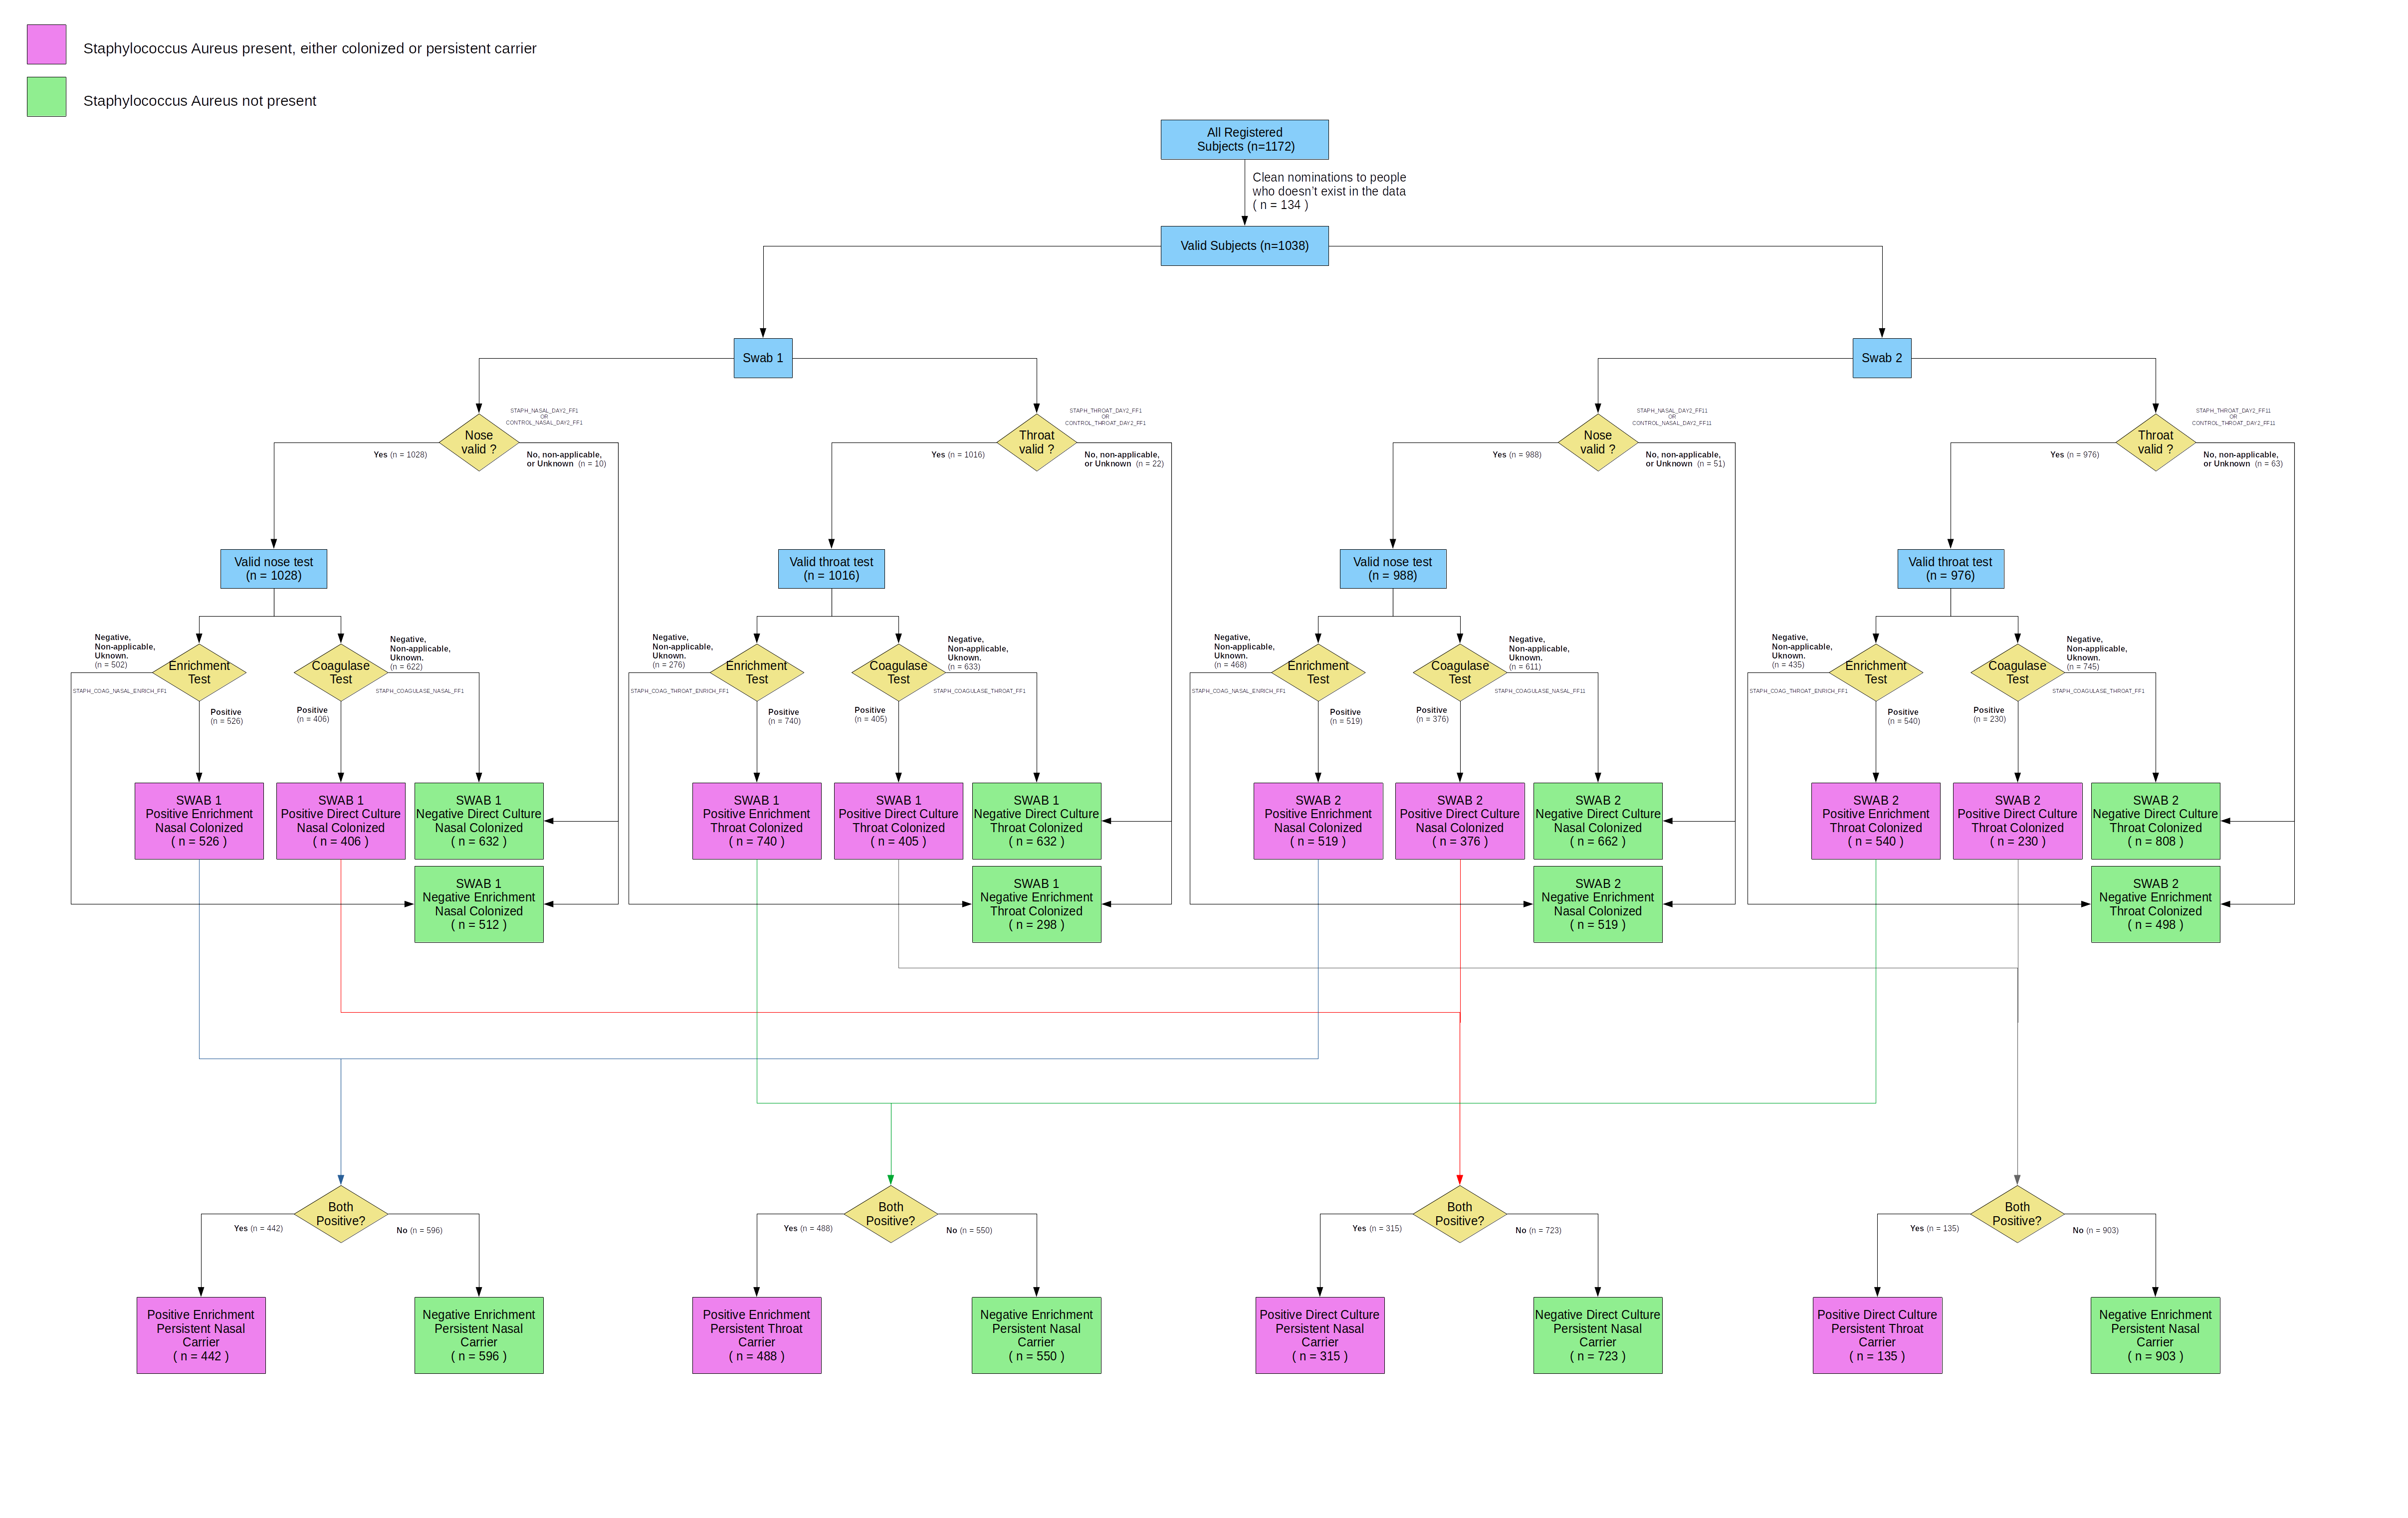
\includegraphics[width=1\textwidth]{../img/figures/carrierDefinition.png}
    \caption{Summarize of the definition of what is a nasal carrier subject. The throat definition follow the same scheme.}
}
\medskip
\end{figure}

	\textit{If we tried a test on the subject which show growing (“NasalGrowth” == “Yes”) and the coagulase test was ALSO positive (“CoagulaseNasal” == “Positive”), then we have a carrier.} \vspace{3 mm}

	The following figures illustrates which are considered carriers in the nose and the throat.\vspace{3 mm}

\input{../img/results/all/CategoricalHeatmap_aureusTable_NasalGrowth_CoagulaseNasal.tex}

\input{../img/results/all/CategoricalHeatmap_aureusTable_ThroatGrowth_CoagulaseThroat.tex}

	There are some minor inconsistencies in the data with this definition, which can be found in the following figures. But in the vast majority of the cases, all the control variables check-out correctly.\vspace{3 mm}

\input{../img/results/all/CategoricalHeatmap_aureusTable_NasalPopulation_CoagulaseNasal.tex}

\input{../img/results/all/CategoricalHeatmap_aureusTable_NasalPopulation_CoagulaseNasal.tex}
	
	We finally added another column to simplify everything, which tells you if you are S. Aureus carrier or not. This is positive if the nose is positive, or the throat is positive, and the other variable is not unknown. This is negative if both of them are negative. If either of them is unknown, this variable is unknown; but at the time of writing this, we have no such cases.\vspace{3 mm}




%%*****************************************
\chapter{Filtering}\label{ch:filtering}
%*****************************************

\section{Intro}

In the previous section we left the original data ready to be imported into any tool that do analysis. Now we have imported this file and we are about to begin our analysis. However we still need to filter by some criteria that we are going to see here. Notice that we don't deal with data stratification here. Later on we will study, for example, men and women separately depending on the context, by class ID, by snuff user status and so on. But that is not filtering. In here we will just take away the rows that we deemed inappropriate for our analysis.\vspace{3 mm}

\section{Filters}

\subsection{By Age}

In Norway, a high-school student is usually between 16 to 19 years old, depending on which grade the student is, but in general they are teenagers within normal teenager years. However we also have some population that are older than 20 years old. Typically these are people with mental disabilities. Because of this, they have an special set of medication, bloodwork statistics, social relationships, and so on that are outliers to our relevant data. As such, we will only consider people who are younger than 20 years old, with age 20 also included.\vspace{3 mm}

We deleted 20 persons like this, and a total of 91 relationships in the overall network. They were nominating a total of 59 people as friends (out), and a total of 50 people were nominating at least one of them as friend (in). They had 18 reciprocal nomination in between them.\vspace{3 mm}

\subsection{By lack of information}

Each person is a row in our data, each variable is a column. There are some columns with missing information. For example, in the BMI variable we have 4 people who doesn't have any BMI values. This doesn't make the whole row for that person worthless because we still have data for many other variables. \vspace{3 mm}

However, in the data that we have in the TSD, there are empty rows, with valid IDs, that either doesn't have any information at all in any of the variables, or have just very few columns with valid data.\vspace{3 mm}

We cannot access the data from the TSD so this part is left blank to fill later, but in here there will be a summary of rows that we had to delete due lack of information.\vspace{3 mm}

\subsection{Final summary}

After taking into account all the previous information, we generated new .csv files, with this filtering criteria, in the folder "../data/filterReady" \vspace{3 mm}

Here is a summary of all the connection that were lost. Of course, all the new friendship information variables that we introduced in the previous chapter \ref{section:friendship_information}, such as popularity for each person, are updated after applying the filter.\vspace{3 mm}

\input{../img/results/all/LatexTable_dataFilteringLogDF.tex}

\input{../img/results/all/Boxplot_missingFriendsDF_Nominations.tex}

\input{../img/results/all/Boxplot_missingFriendsDF_Popularity.tex}

\section{Updating variables}

After deleting these rows, we need to update some variables again, similarly as we did during the data cleaning process. As in re-assigning IDs so everybody has consecutive IDs and the friendship matrices indexes match with the person ID, re-calculating the friendship information in the phenotype table, re-construct the network matrices to keep up with the ID changes.



\vspace{3 mm}

\include{Chapters/ChapterGENERAL}
%\include{Chapters/ChapterVARIABLES}


\newpage

\printindex

\newpage

\end{document}


%\ (!!) You need to compile twice to make the internal references to work
